%% 
%% Copyright 2007-2019 Elsevier Ltd
%% 
%% This file is part of the 'Elsarticle Bundle'.
%% ---------------------------------------------
%% 
%% It may be distributed under the conditions of the LaTeX Project Public
%% License, either version 1.2 of this license or (at your option) any
%% later version.  The latest version of this license is in
%%    http://www.latex-project.org/lppl.txt
%% and version 1.2 or later is part of all distributions of LaTeX
%% version 1999/12/01 or later.
%% 
%% The list of all files belonging to the 'Elsarticle Bundle' is
%% given in the file `manifest.txt'.
%% 
%% Template article for Elsevier's document class `elsarticle'
%% with harvard style bibliographic references

% \documentclass[preprint,12pt]{elsarticle}
\documentclass[5p,times]{elsarticle}

%% Use the option review to obtain double line spacing
%% \documentclass[preprint,review,12pt]{elsarticle}

%% Use the options 1p,twocolumn; 3p; 3p,twocolumn; 5p; or 5p,twocolumn
%% for a journal layout:
%% \documentclass[final,1p,times]{elsarticle}
%% \documentclass[final,1p,times,twocolumn]{elsarticle}
%% \documentclass[final,3p,times]{elsarticle}
%% \documentclass[final,3p,times,twocolumn]{elsarticle}
%% \documentclass[final,5p,times]{elsarticle}
%% \documentclass[final,5p,times,twocolumn]{elsarticle}

%% For including figures, graphicx.sty has been loaded in
%% elsarticle.cls. If you prefer to use the old commands
%% please give \usepackage{epsfig}

%% The amssymb package provides various useful mathematical symbols
\usepackage{amssymb}
%% The amsthm package provides extended theorem environments
\usepackage{amsthm}

\usepackage[fleqn]{amsmath}
\usepackage{multirow}
\tolerance=1000

%% The lineno packages adds line numbers. Start line numbering with
%% \begin{linenumbers}, end it with \end{linenumbers}. Or switch it on
%% for the whole article with \linenumbers.
%% \usepackage{lineno}

\journal{Parallel Computing}

\begin{document}

\begin{frontmatter}

%% Title, authors and addresses

%% use the tnoteref command within \title for footnotes;
%% use the tnotetext command for theassociated footnote;
%% use the fnref command within \author or \address for footnotes;
%% use the fntext command for theassociated footnote;
%% use the corref command within \author for corresponding author footnotes;
%% use the cortext command for theassociated footnote;
%% use the ead command for the email address,
%% and the form \ead[url] for the home page:
\title{Title}
% \tnotetext[label1]{}
\author[label1]{Hongbin Liu}
\author[label1]{Hu Ren\corref{cor1}}
\ead{renhu@mail.nsccwx.cn}
% \ead[url]{home page}
% \fntext[label2]{214000}
\cortext[cor1]{Corresponding author.}
% \address{National Supercomputing Center in Wuxi}
% \fntext[label3]{National Supercomputing Center in Wuxi}

\title{UNAT: an UNstructured Acceleration Toolkit and its implementation on SW26010 many-core processor}

%% use optional labels to link authors explicitly to addresses:
% \author[label1]{Hongbin Liu}
\author[label1,label2]{Hanfeng Gu}
\author[label1]{Fei Gao}
\author[label1,label2]{Haohuan Fu}
\author[label1,label2]{Guangwen Yang}
\address[label1]{National Supercomputing Center in Wuxi}
\address[label2]{Tsinghua University}

% \author{}

% \address{}

\begin{abstract}
% Text of abstract

Unstructured grids are increasingly popular in scientific and engineering computation for their geometrical flexibility. However, high fidelity applications based on unstructured grids are still time-consuming, no matter for programming or running. For example, the cost of large eddy simulation for fluid flow is still unacceptable for researchers, which promotes the development of modern supercomputers. In the meantime, the diversity of innovatory hardware architectures increases the complexity and difficulty of machine-specific optimization and code maintenance.

Hence the aim of this work is to develop an efficient UNstructured Acceleration Toolkit (UNAT), which provides friendly high-level programming interfaces and elaborate lower level implementation on the target hardware to get nearly hand-optimized performance. At present state, two efficient strategies, Multi-Level Blocks method and Row-Subsections method, are designed and implemented on Sunway architecture. Irregular memory access and write conflict issue of unstructured mesh have been handled by partitioning, coloring and other hardware-specific techniques. Moreover, a data-reuse mechanism is developed to increase the compute-intensity and alleviate the memory bandwidth bottleneck.

We select a representative operator, SpMV, as a performance benchmark of UNAT across different data layouts and different matrix formats. Experimental results show that the speed-ups reach up to 26 compared to single MPE, and the utilization ratio tests indicate the capability of achieving nearly hand-optimized performance.
\end{abstract}

%%Graphical abstract
% \begin{graphicalabstract}
%\includegraphics{grabs}
% \end{graphicalabstract}

%%Research highlights
% \begin{highlights}
% \item Research highlight 1
% \item Research highlight 2
% \end{highlights}

\begin{keyword}
%% keywords here, in the form: keyword \sep keyword
UNAT \sep Unstructured Mesh \sep Domain Specific Language \sep Sunway architecture
%% PACS codes here, in the form: \PACS code \sep code

%% MSC codes here, in the form: \MSC code \sep code
%% or \MSC[2008] code \sep code (2000 is the default)

\end{keyword}

\end{frontmatter}

%% \linenumbers

%% main text
\section{Introduction}
\label{Introduction}

Among all kinds of mesh types, unstructured meshes are dominant in engineering simulation scenarios and play important role in scientific computations. Discretization methods such as Finite Element Method (FEM) and Finite Volume Method (FVM), are well performed for decades on unstructured meshes for solving various kinds of PDEs. However, high fidelity applications based on unstructured grids are still time-consuming, no matter for programming or running. The fluid flow simulation, a typical application mostly utilizing FVM discretization on unstructured mesh, notably relies on huge computing power for high fidelity results. On the other hand, as high performance computers progressively increase the computing capacity, the complexity of hardware architectures and the programming difficulty form a high barrier to entry for domain developers.

With the advent of novel processor architectures, especially many-core ones, the parallel programming models experienced an explosive growth \cite{b1}. Careful programming design and optimization are essential to take advantage of the full potential of emerging parallel high performance systems \cite{b2}. Compared to the multi-core architectures, processors employing many-core architecture such as the Intel Many Integrated Core (MIC) processors and NVIDIA GP-GPUs become the most popular HPC platform among all the newest HPCs on the Top500 list. Consequently, along with the traditional pure parallel programming models like MPI and OpenMP, platform-specific models for heterogeneous many-core architecture including CUDA and OpenCL formed an abundant family with a number of distinct and confusing characteristics. More intricate details of new architectures must be noted specially to attain optimal performance \cite{b3}, which results in the extremely high development costs and extra maintenance difficulties for domain developers.

Specifically, handling the inherent problems in unstructured mesh-base computations requires more effort on many-core platforms. With a general abstraction, unstructured computation can be deemed as calculations performed on an adjacent graph. As we all know, the start-vertices/owners and end-vertices/neighbors of edges cannot be stored consecutively in the same time, so irregular and indirect data access is inevitable in efficient unstructured computation. Fine-grained parallel computing on many-core architecture amplifies this problem. For example, the indirect data addressing may stride a number of threads and result in the inefficient memory access on the modern Non-Uniform Memory Architecture (NUMA) configuration\cite{b4}. Simultaneously, race condition problem is also prominent, since the high concurrency of threads makes the general technics such as atomic primitive expensive\cite{b6}\cite{b6-6}. Further, irregular data access also means a large percent of ineffective data in a single cache line\cite{b7}\cite{b8-8}\cite{b9-9}, which reduces the effective memory bandwidth. To address those problems, a lot of optimizations practiced on shared-memory multi-core and many-core platforms are reported. The strategies can be classified into five main categories:
\begin{enumerate}
\item Improve the locality of data sets or tasks to enable better memory and cache efficiency. The basic methods like Reverse Cuthill-Mckee (RCM) method that minimized the bandwidth of the adjacent matrix\cite{b7}\cite{b8-8}\cite{b14-14}, and partition methods\cite{b4}\cite{b12-12} using high-end graph partition libraries like METIS/ParMETIS and Scotch/Pt-Scotch\cite{b2} are both widely used to improve data locality. Cache level and size-aware partition strategies\cite{b2}\cite{b4}\cite{b12-12}, as well as ones caring about the algorithm itself\cite{b12-12}, are reported to give more optimal performance. 
\item Color tasks or data sets to dig parallelism and avoid race condition\cite{b2}\cite{b4}\cite{b7}\cite{b8-8}\cite{b18-18}. Although coloring algorithm is not always more efficient than atomic primitive, it is still valuable when the hardware level atomic primitive is absent.\cite{b18-18}.
\item Tile the data set and prefetch at runtime. Tiling enables the calculation process to locate necessary data sets dependent on and reduce the waste of memory bandwidth. Some Intel MIC processors provide software prefetching with a given distance that reduces the cache miss in irregular and indirect data access\cite{b7}\cite{b8}.
\item Vectorization. A gather-compute-scatter model with vectorization was reported in some works applied to irregular and indirect data access\cite{b7}\cite{b21-21}. However, in most real cases unstructured mesh applications are bandwidth-bounded regardless of using vectorization or not\cite{b21-21}.
\item Reuse data or eliminate intermediate results to reduce memory bandwidth cost. The unstructured computation give much pressure to the limited bandwidth especially on many-core platforms, so strategies like loop fusion\cite{b22-22} were taken to alleviate this kind of adverse impact.
\end{enumerate}

To handle the problems on unstructured computation addressed above, we developed an accelerating tool UNAT, an abbreviation of unstructured mesh-based accelerating toolkit, which provides friendly high-level programming interface and at the same time elaborated lower level architecture-aware implementation attaining nearly hand-optimized performance on the target hardware. A number of research projects have implemented similar or related programming frameworks. A comparable counterpart OP2\cite{b2}, developed in Oxford University, aimed at achieving performance portability on different back-end hardware platforms without the intervention of the domain application programmer using unstructured meshes. As OP2 utilizes a code generation strategy, our work adopts a functional programming philosophy that enables users to code in sequential style with general languages like C. There are also some points in common. For example, both OP2 and UNAT separate data, map and operations into decoupled components and adopt a preprocess-access-execute procedure design. The detail of UNAT design will be described in Sec. \ref{sec:design}.

At the present stage, UNAT is implemented and tested on the SW26010 processor, the one used to construct the world’s 100-peta-flops supercomputer Sunway Taihulight. In this work, we perform two kinds of optimization strategies on SW26010 platform. The first one is a Multi-Level Blocks (MLB) based implementation that emphasizes data locality consistent with the cache size and hierarchy, and the second one is an accurate tiling based implementation named Row-Subsections (RSS) that adopts a light-weight preprocessing and is kernel-adaptive. Data segment with coloring algorithm is used in the RSS implementation to avoid race condition. The implementations of both optimizations are described in detail in Sec. \ref{sec:parallel}. Technics specified on the SW26010, such as the accurate and programmable caching and memory accessing, are also utilized in our implementations. Moreover, a data-reuse mechanism is developed to increase the compute-intensity and alleviate the memory bandwidth bottleneck, which will be presented in Sec. \ref{sec:design}. Performance results and discussions will be presented in the Sec. \ref{sec:perf}.

\section{Design and API}
\label{sec:design}

\subsection{Abstraction and API}

Unstructured computation can actually be abstracted as calculations on an graph. For example, in FEM discretization, a graph is constructed with the mesh nodes as the graph vertices and the mesh edges as the graph edges. In FVM discretization, the graph can be extracted with the mesh cells as the graph vertices and the cell faces as the edges. Thanks to such an abstraction, the connectivity of unstructured mesh can be represented as a graph or a sparse adjacency matrix.

The computation over a graph or an adjacency matrix can be decomposed into three parts: data sets, connectivity and operations over data sets, which leads to the design of UNAT API. The UNAT API supports C/C++ and Fortran programming language and here we adopt the C/C++ API in this paper. As the combination of frequently appeared operations, interpolation and integration, in unstructured computation, Sparse Matrix Vector multiplication (SpMV) operation is adopted to illustrate the UNAT API in this paper. The matrix $A$ could be stored with multiple sparse matrix formats such as Lower-Diagonal-Upper(LDU), Compressed Sparse Row(CSR), Coordinate list(COO), et al. UNAT supports both LDU and COO formats.

The data sets can be defined on any entities of unstructured mesh such as the nodes, edges, faces and other elements. The associated data could be coordinates, velocities, coefficients or weights. As for the specific operation SpMV, The associated data are coefficients and vectors, which are defined respectively on the non-zeros of matrix and row/column. Then the data sets of SpMV with LDU format can be defined using the UNAT API as shown in Fig. \ref{dataset}.
\begin{figure}[htbp]
	\centerline{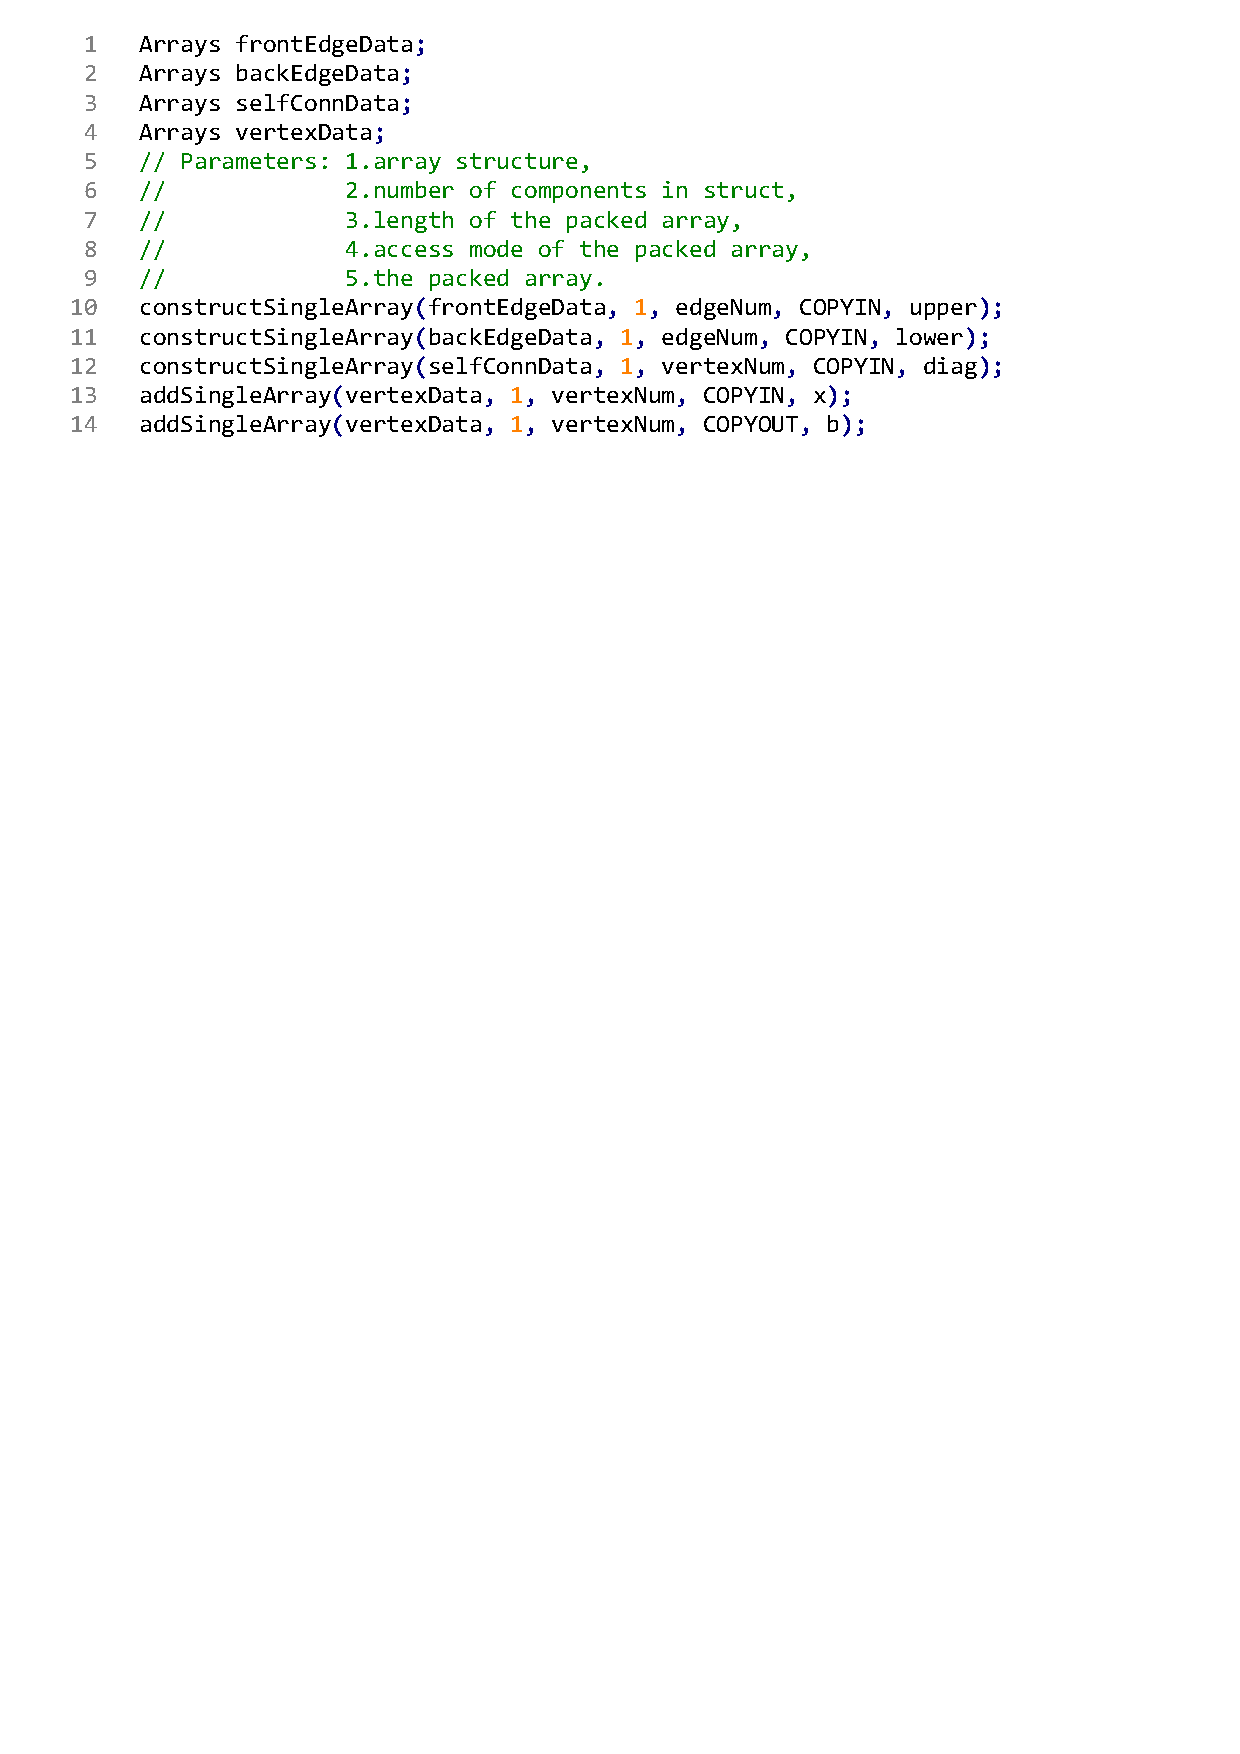
\includegraphics[width=0.49\textwidth]{data-set.pdf}}
	\caption{Definition of data sets with UNAT API(LDU).}
	\label{dataset}
\end{figure}
Four variables, $frontEdgeData$, $backEdgeData$, $selfConnData$ and $vertexData$, indicate the non-zeros in the upper triangle $upper$, lower triangle $lower$, diagonal line $diag$ and vectors $x$/$b$. The struct $Arrays$ consists of multiple arrays with Struct of Arrays (SoA) data layout such as $x$ and $b$ in the $vertexData$. While for $x$ and $b$, the data is stored with Arrays of Structs layout, and then the struct $Arrays$ has a Struct of Arrays of Structs (SoAoS) layout as shown in Fig. \ref{soaos}.

\begin{figure}[htbp]
	\centerline{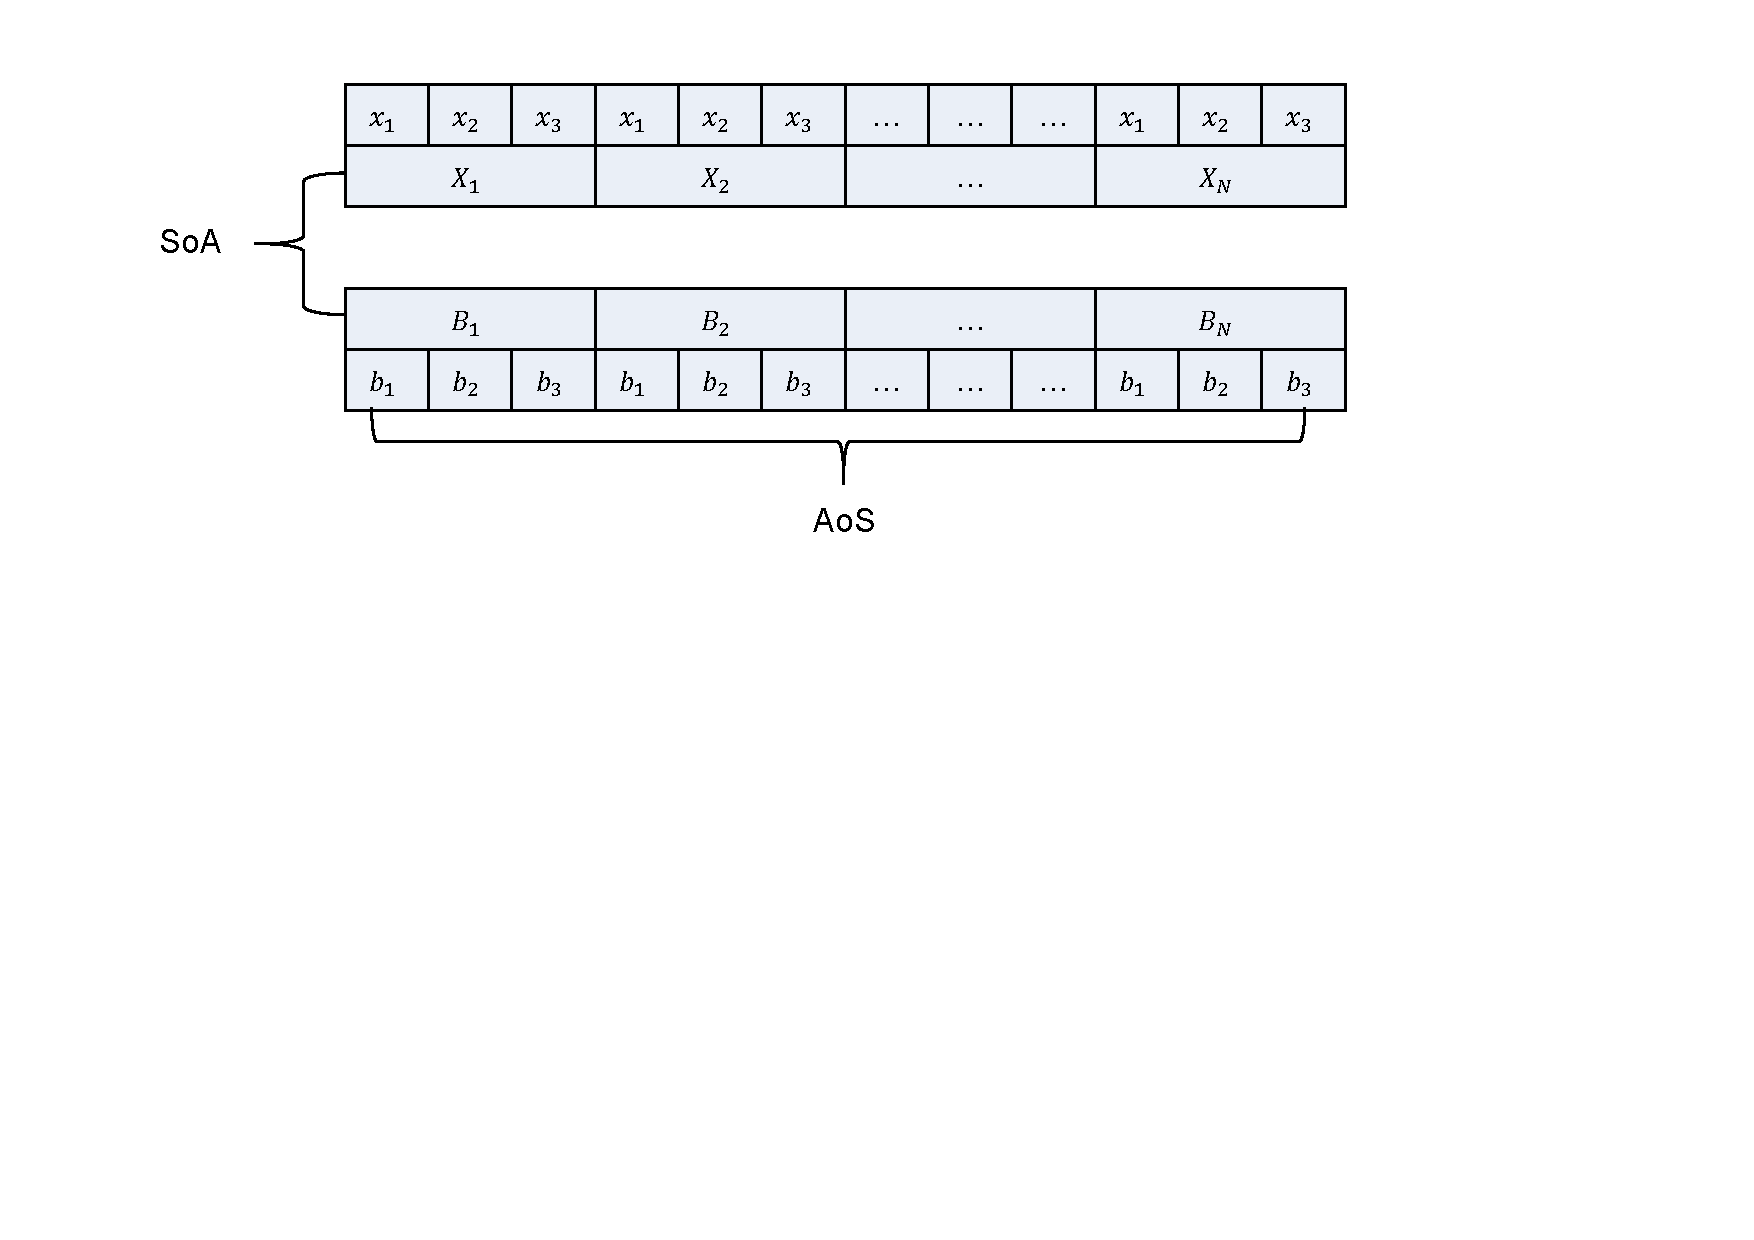
\includegraphics[width=0.49\textwidth]{SoAoS.pdf}}
	\caption{Diagram of SoAoS layout in struct $Arrays$.}
	\label{soaos}
\end{figure}

The binding process under COO format is similar except for the absence of lower triangle and diagonal line and the codes are as shown in Fig. \ref{dataset-coo}. It should be noted that the values of $edgeNum$ and $vertexNum$ are different from the LDU format. The float array $edge$ gives the non-zeros of matrix $A$.

\begin{figure}[htbp]
	\centerline{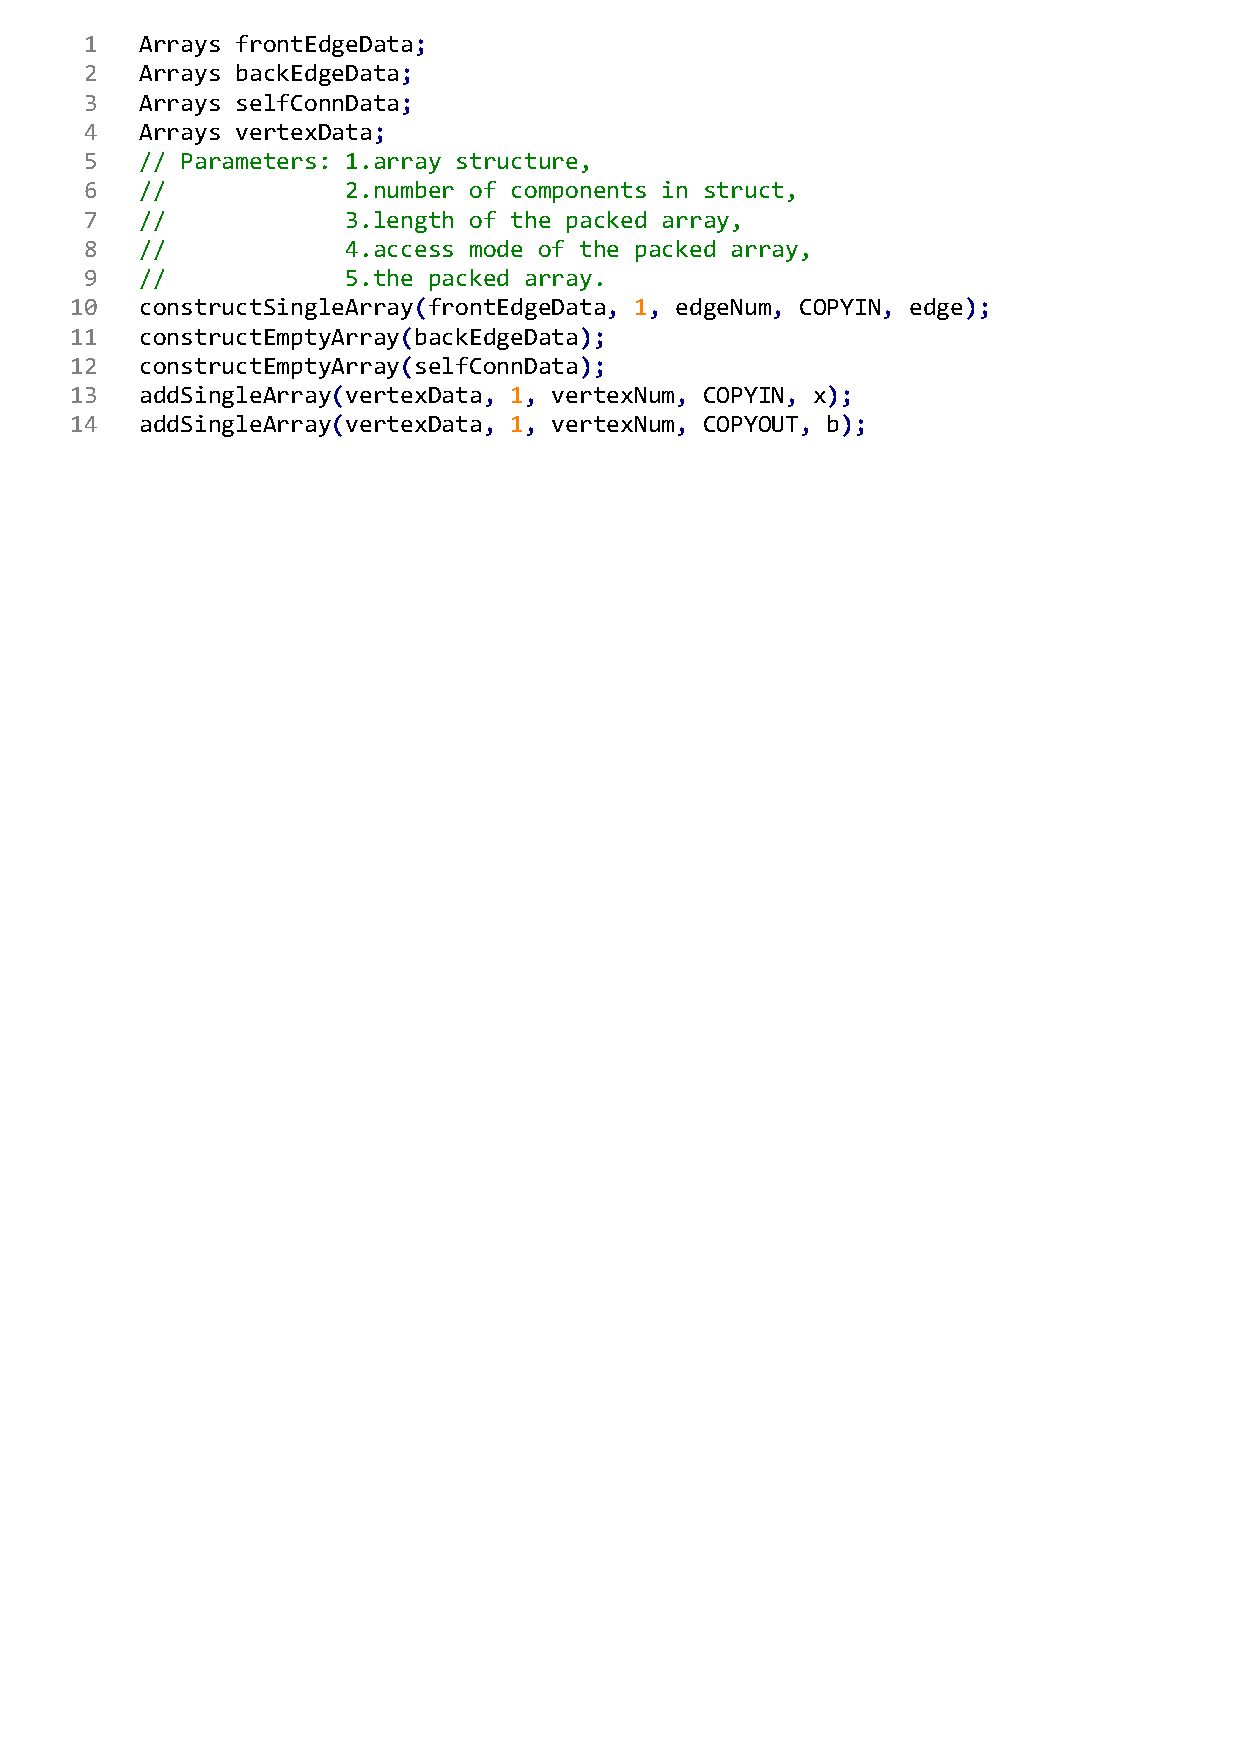
\includegraphics[width=0.49\textwidth]{data-set-coo.pdf}}
	\caption{Definition of data sets with UNAT API(COO).}
	\label{dataset-coo}
\end{figure}

As for the connectivity, class $Topology$ record the map between different data sets and class $Iterator$ utilize partition, tiling or coloring algorithm to improve the data locality. We provide two iterators for different application scenarios and this will be discussed in detail in the next chapter. The construction and prepossessing of connectivity with UNAT API are as shown in Fig. \ref{connectivity}.
\begin{figure}[htbp]
	\centerline{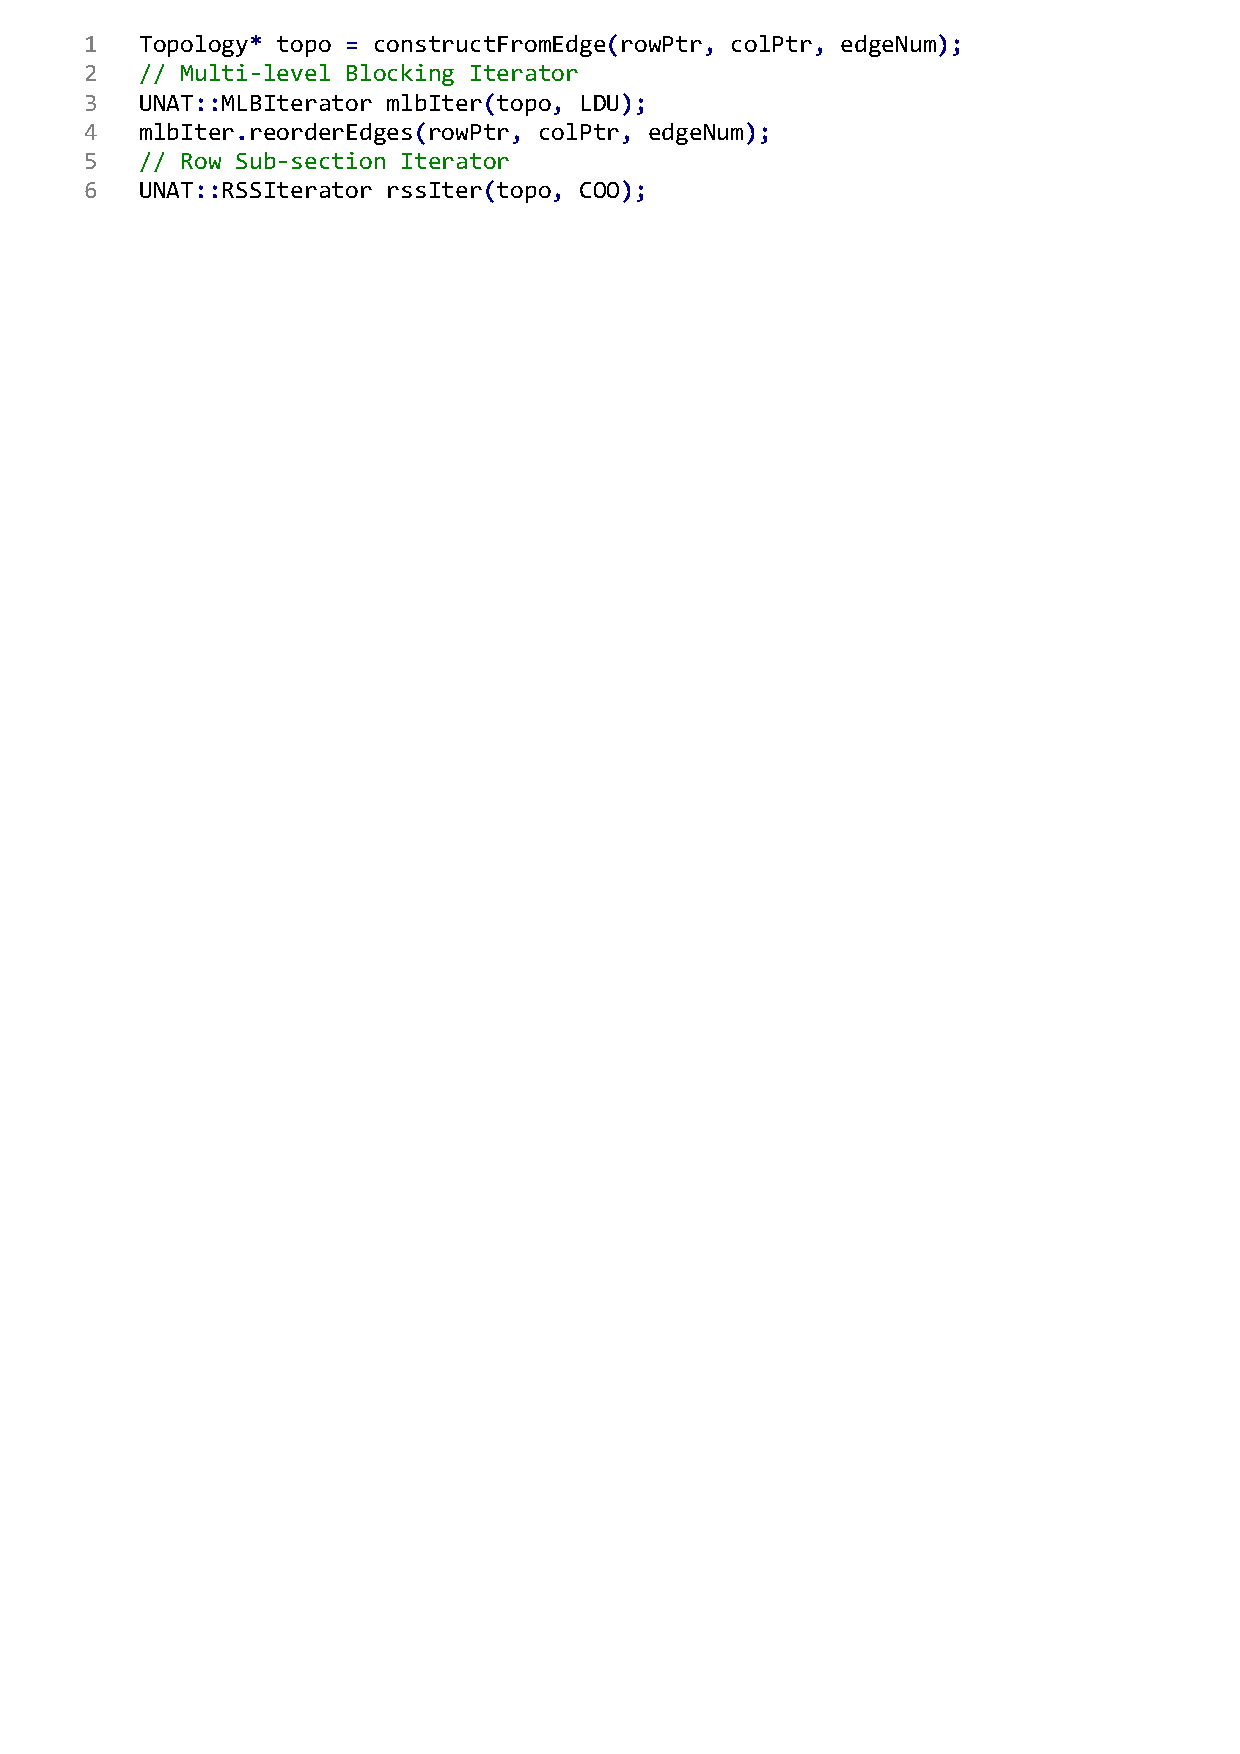
\includegraphics[width=0.49\textwidth]{connectivity.pdf}}
	\caption{Definition of connectivity with UNAT API}
	\label{connectivity}
\end{figure}
The class $Topology$ get the row and column indices of LDU format, while both LDU and COO format are available for iterator.

Benefiting from the above abstraction, the operation with UNAT API is defined analogously as shown in Fig. \ref{spmv} and there are two main differences. Firstly, the computation of lower triangle and upper triangle is separated for the compatibility of different matrix format, because the lower triangle is absent in COO format; In addition, the exist of inner loop origins from the AoS data layout.
\begin{figure}[htb]
	\centerline{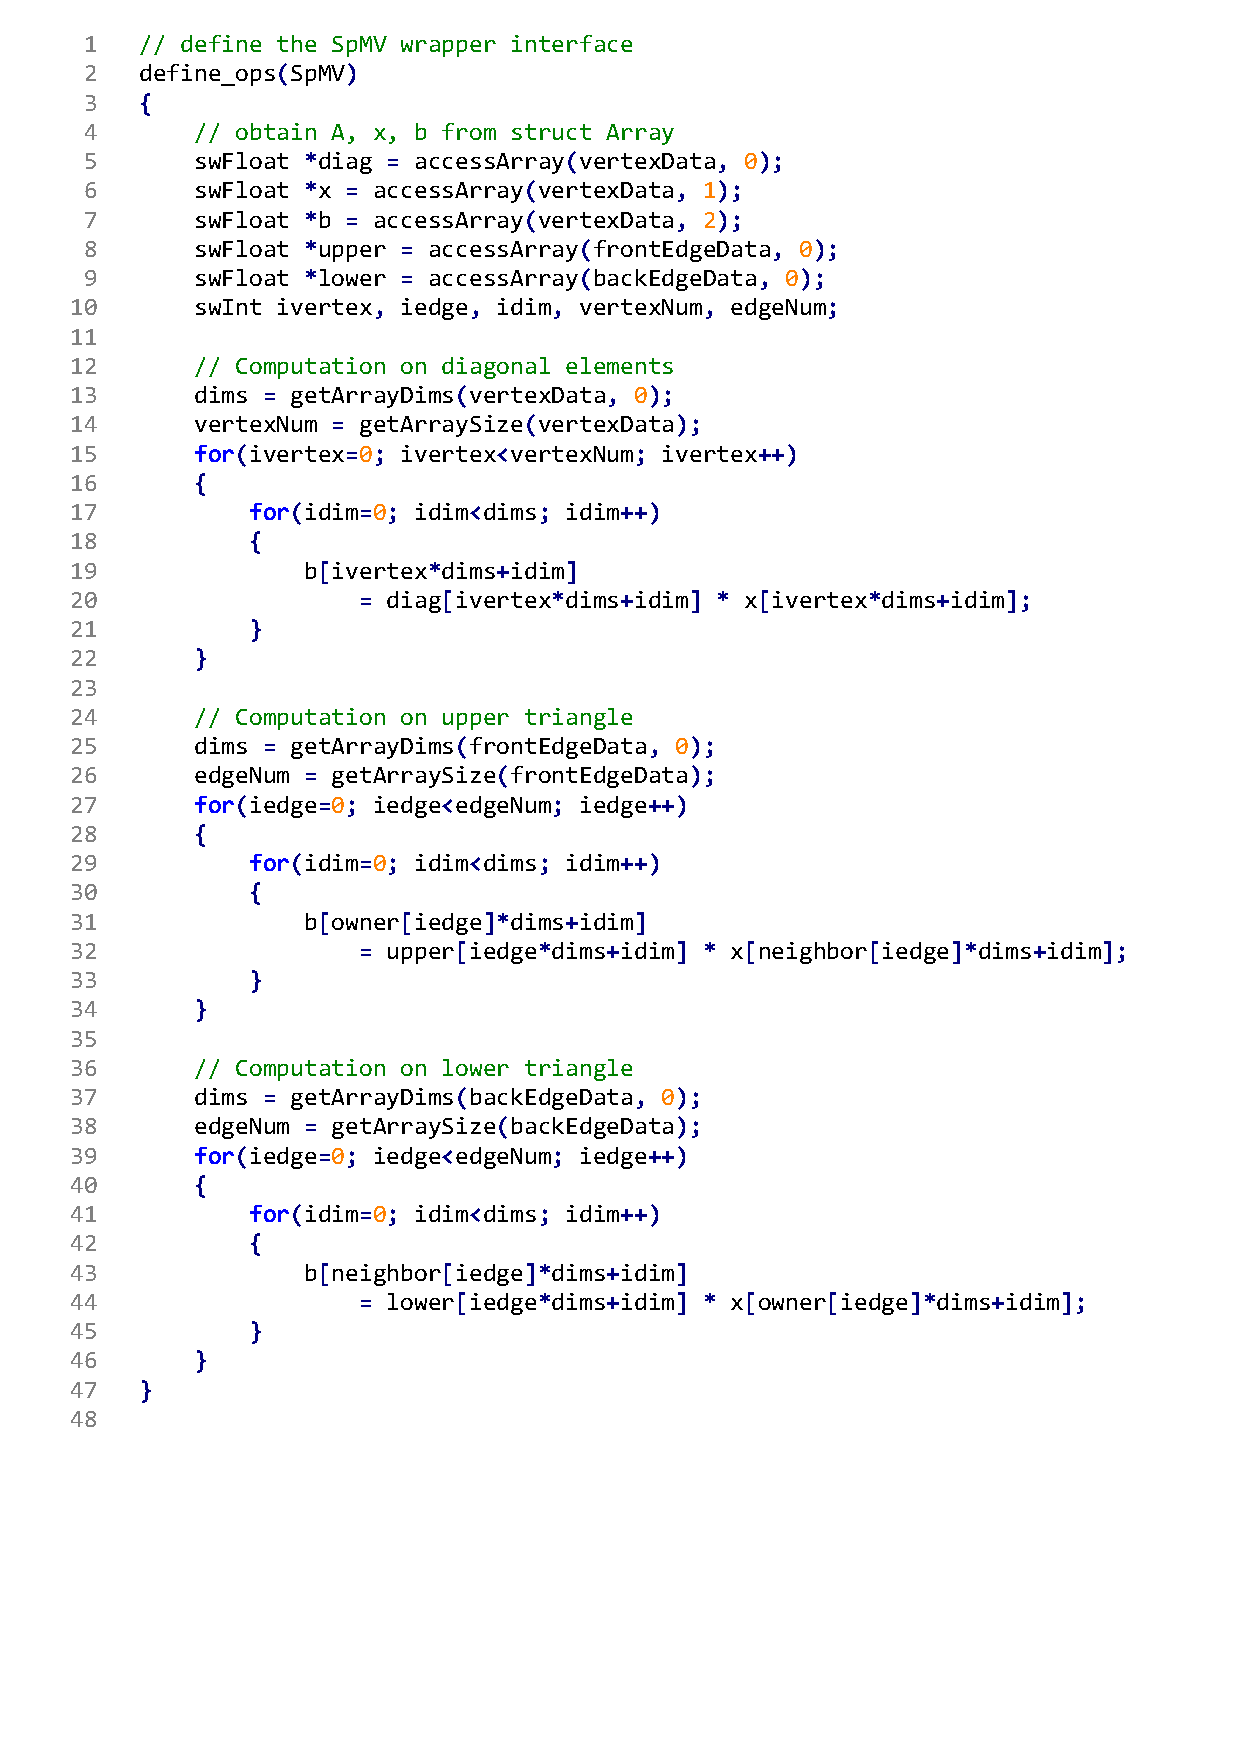
\includegraphics[width=0.49\textwidth]{spmv.pdf}}
	\caption{Definition of SpMV operation with UNAT API}
	\label{spmv}
\end{figure}

Finally, after the definition of data sets, connectivity and operation, we need to couple data sets and operations into a $CoupledOperator$ and then pass it to $Iterator$ for execution as shown in Fig. \ref{iteration}. The number $1$ in the parameter list indicate that only one operation, SpMV, is included in the coupled operator. $slave_SpMV$ and $SpMV$ are actually the same function pointer, which is defined in Fig. \ref{spmv}. $paraData$ is a independent variable for storing constant parameters such as viscosity coefficient or specific heat. The detail of iteration will be discussed in the next chapter.
\begin{figure}[htbp]
	\centerline{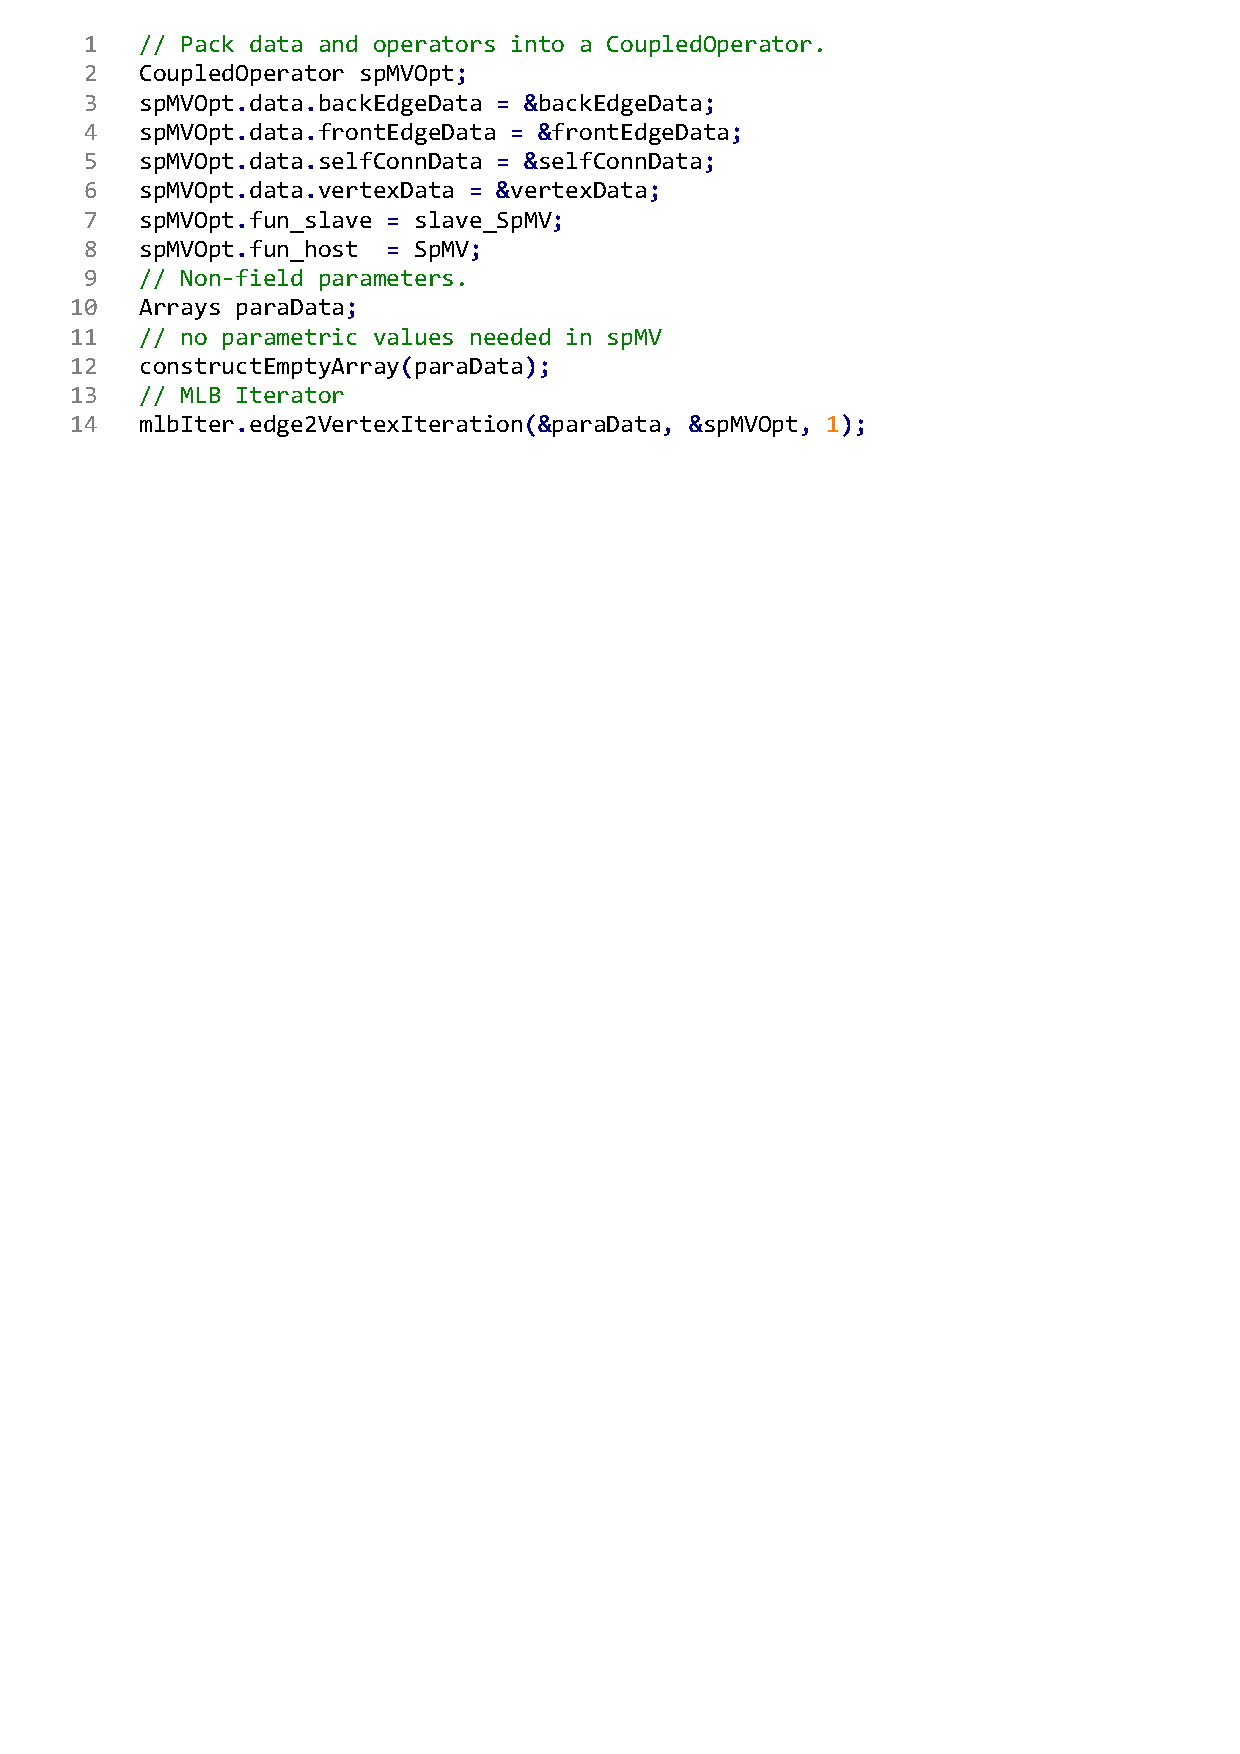
\includegraphics[width=0.49\textwidth]{iteration.pdf}}
	\caption{Definition of iterator with UNAT API}
	\label{iteration}
\end{figure}

It is clear that about 50 lines additional code is needed for the parallelization of one specific operation. This domain-specific language hides the parallel implementation and alleviate the programming difficulty for the domain engineers.

\subsection{CoupledOperator}

The cache of many-core processor is precious for its low latency and rareness. The efficient utilization of cache can extremely alleviate the pressure of memory bandwidth. In the operators of current applications, a number of local arrays are allocated and stored in the memory for convenience. It is almost impossible to load these arrays thoroughly to the limited cache unless the block size is small enough. Although the decomposition of operators can reduce the number of local arrays and fulfill the demand of cache capacity, some intermediate arrays need to be stored and accessed repeatedly, which increases the pressure of memory bandwidth. On the other hand, all arrays have their own lifespans, so it is uneconomical to keep them all "active" in cache during the whole period of operators.

Therefore, we design a data-reuse mechanism to integrate these decomposed sub-operators into coupled operator. Fig. \ref{coupledoperator} presents the diagram of coupled operator.
\begin{figure}[htbp]
	\centerline{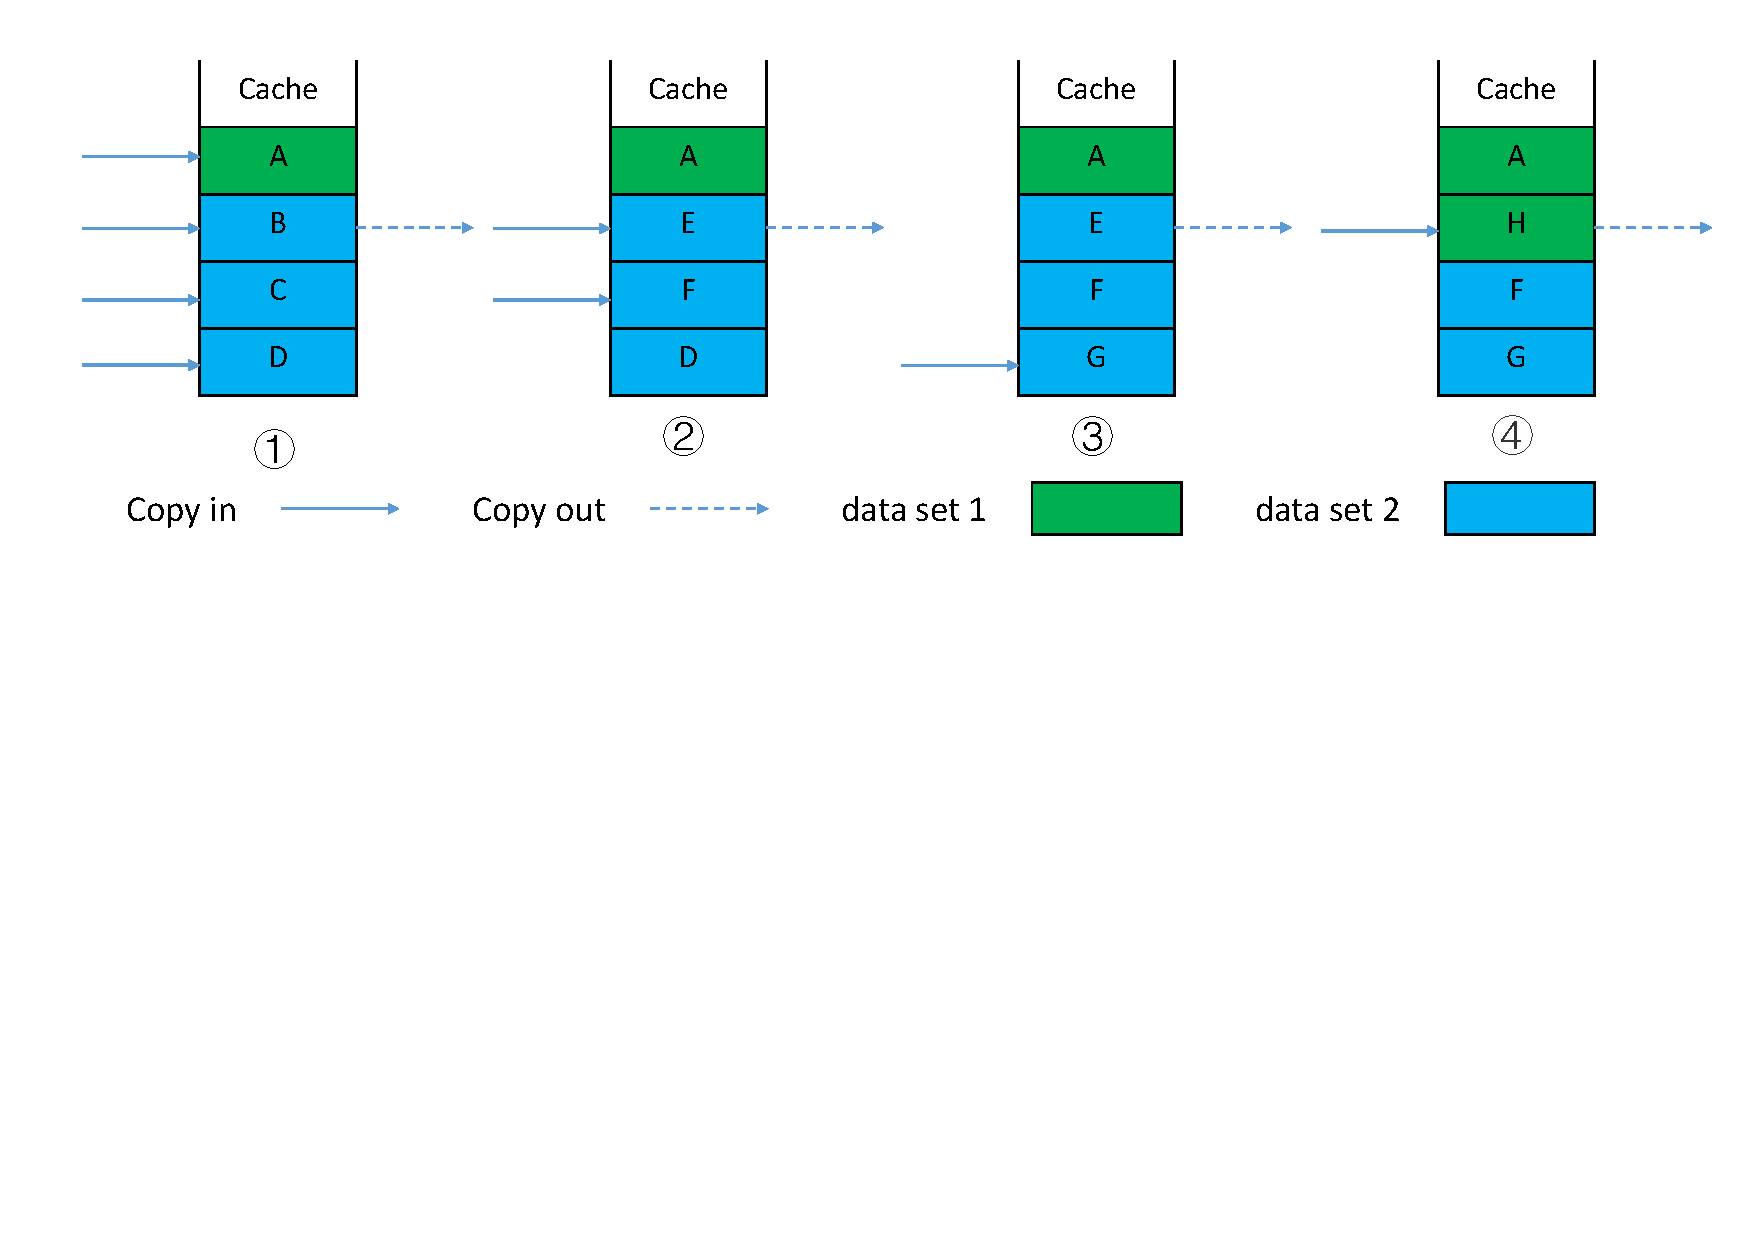
\includegraphics[width=0.49\textwidth]{coupledoperator.pdf}}
	\caption{Data-reuse mechanism in coupled operator}
	\label{coupledoperator}
\end{figure}
The original operator consists of 8 intermediate arrays ($A...H$) during the computation process. Two of them, $A$ and $H$, are data corresponding to the data set 1 of adjacency matrix and the others are data corresponding to the data set 2. By analyzing the lifespan of arrays, The maximum number of correlative arrays is 4. Firstly, arrays $A$, $B$, $C$ and $D$ are loaded into LDM through direct memory access, and then array $B$ is copied out after computing. In the next step, the space of $B$ and $C$ are occupied by new arrays $E$ and $F$ while $A$ and $D$ are reused. These two steps can be declared as shown in Fig. \ref{coupledoperator_code}.
\begin{figure}[htbp]
	\centerline{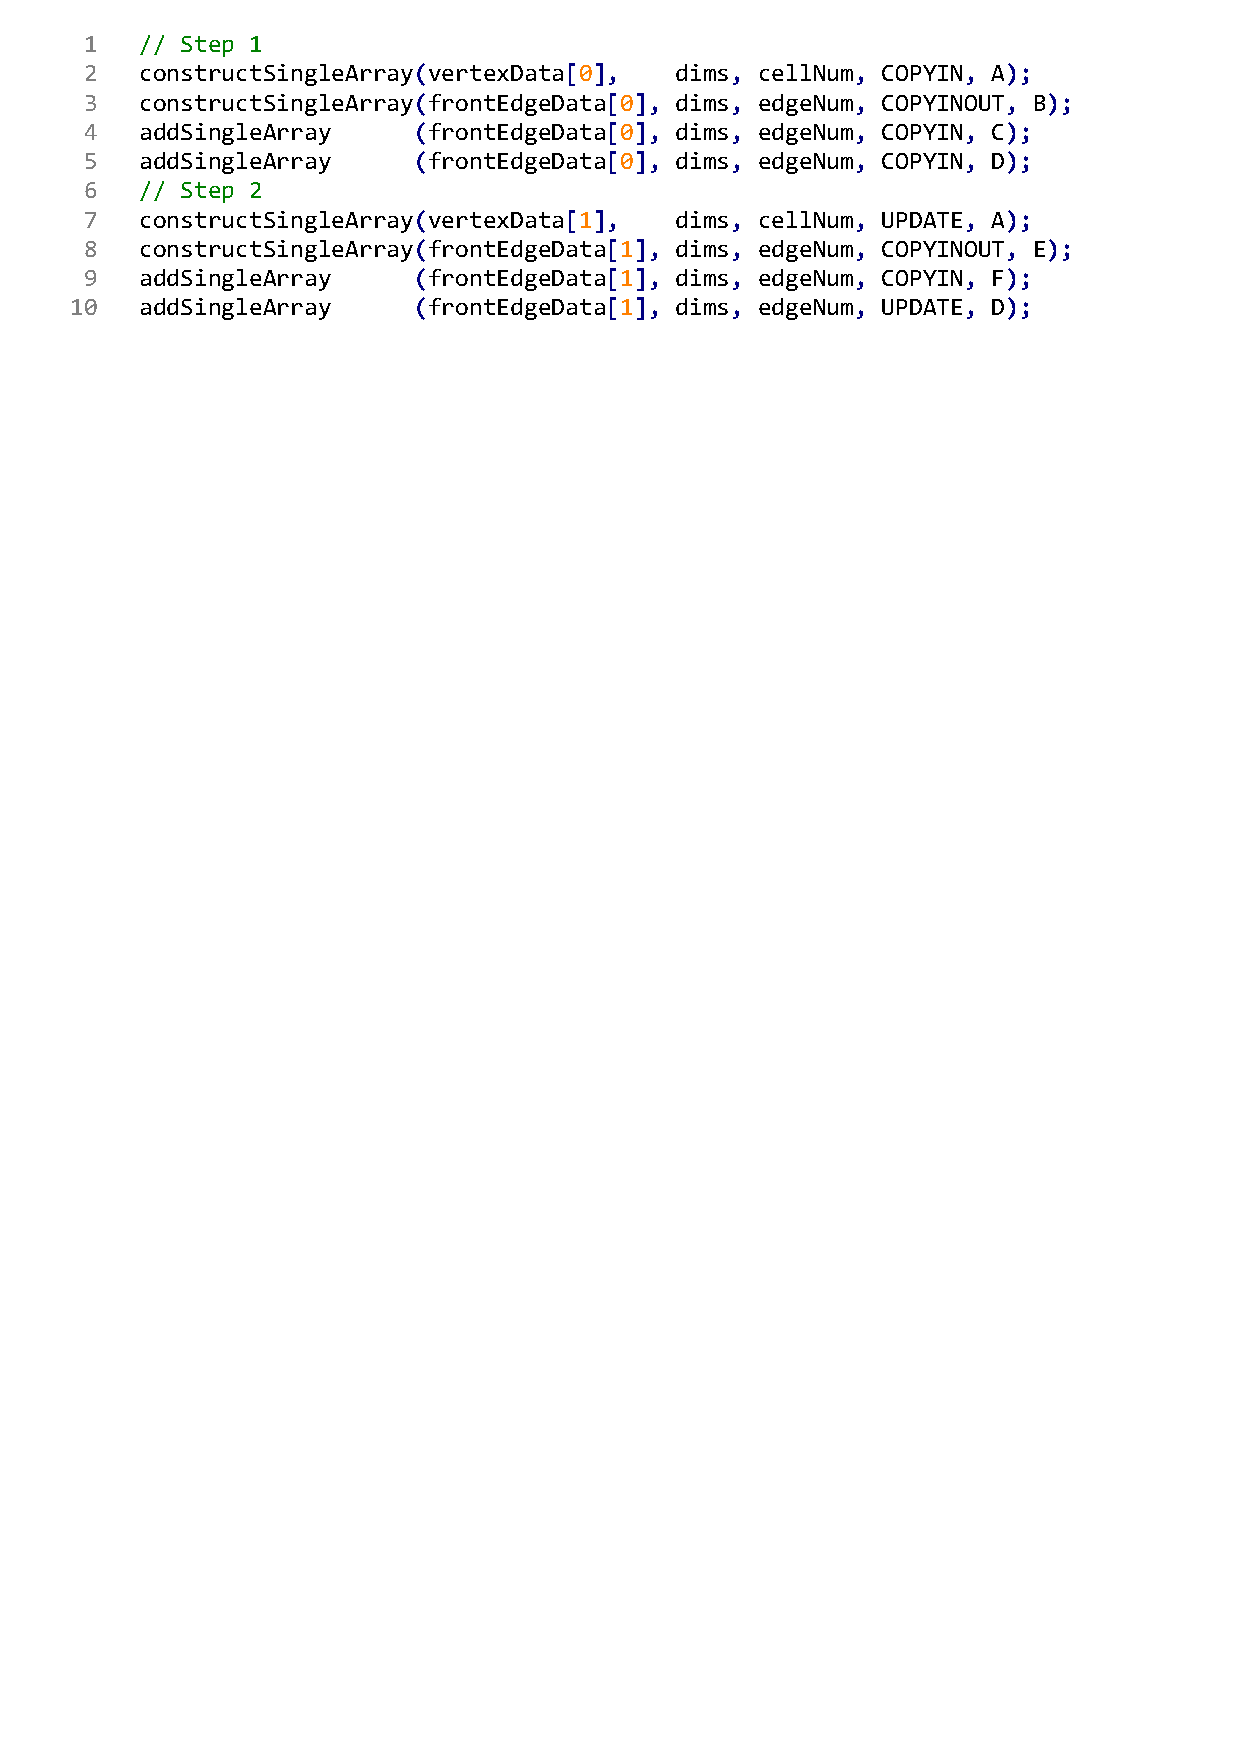
\includegraphics[width=0.49\textwidth]{coupledoperator_code.pdf}}
	\caption{Codes example of coupled operator}
	\label{coupledoperator_code}
\end{figure}
The intrinsic word $update$ indicates the binding array has been stored in the cache without further memory access. It is important to note that $copyout$ may imply the same meaning with $update$. For example, the array $E$ in step \textcircled{3} does not need any direct memory access since $copyin$ has been performed in step \textcircled{2}.

\section{Parallelization Strategy}
\label{sec:parallel}

\subsection{SW26010 Many-core processor}

The SW26010 many-core processor is the basic component unit of the Sunway TaihuLight supercomputer, which is designed by Shanghai High Performance IC Design Center. The detail of Sunway architecture is illustrated in Fig. \ref{sw26010}.
\begin{figure}[htbp]
\centerline{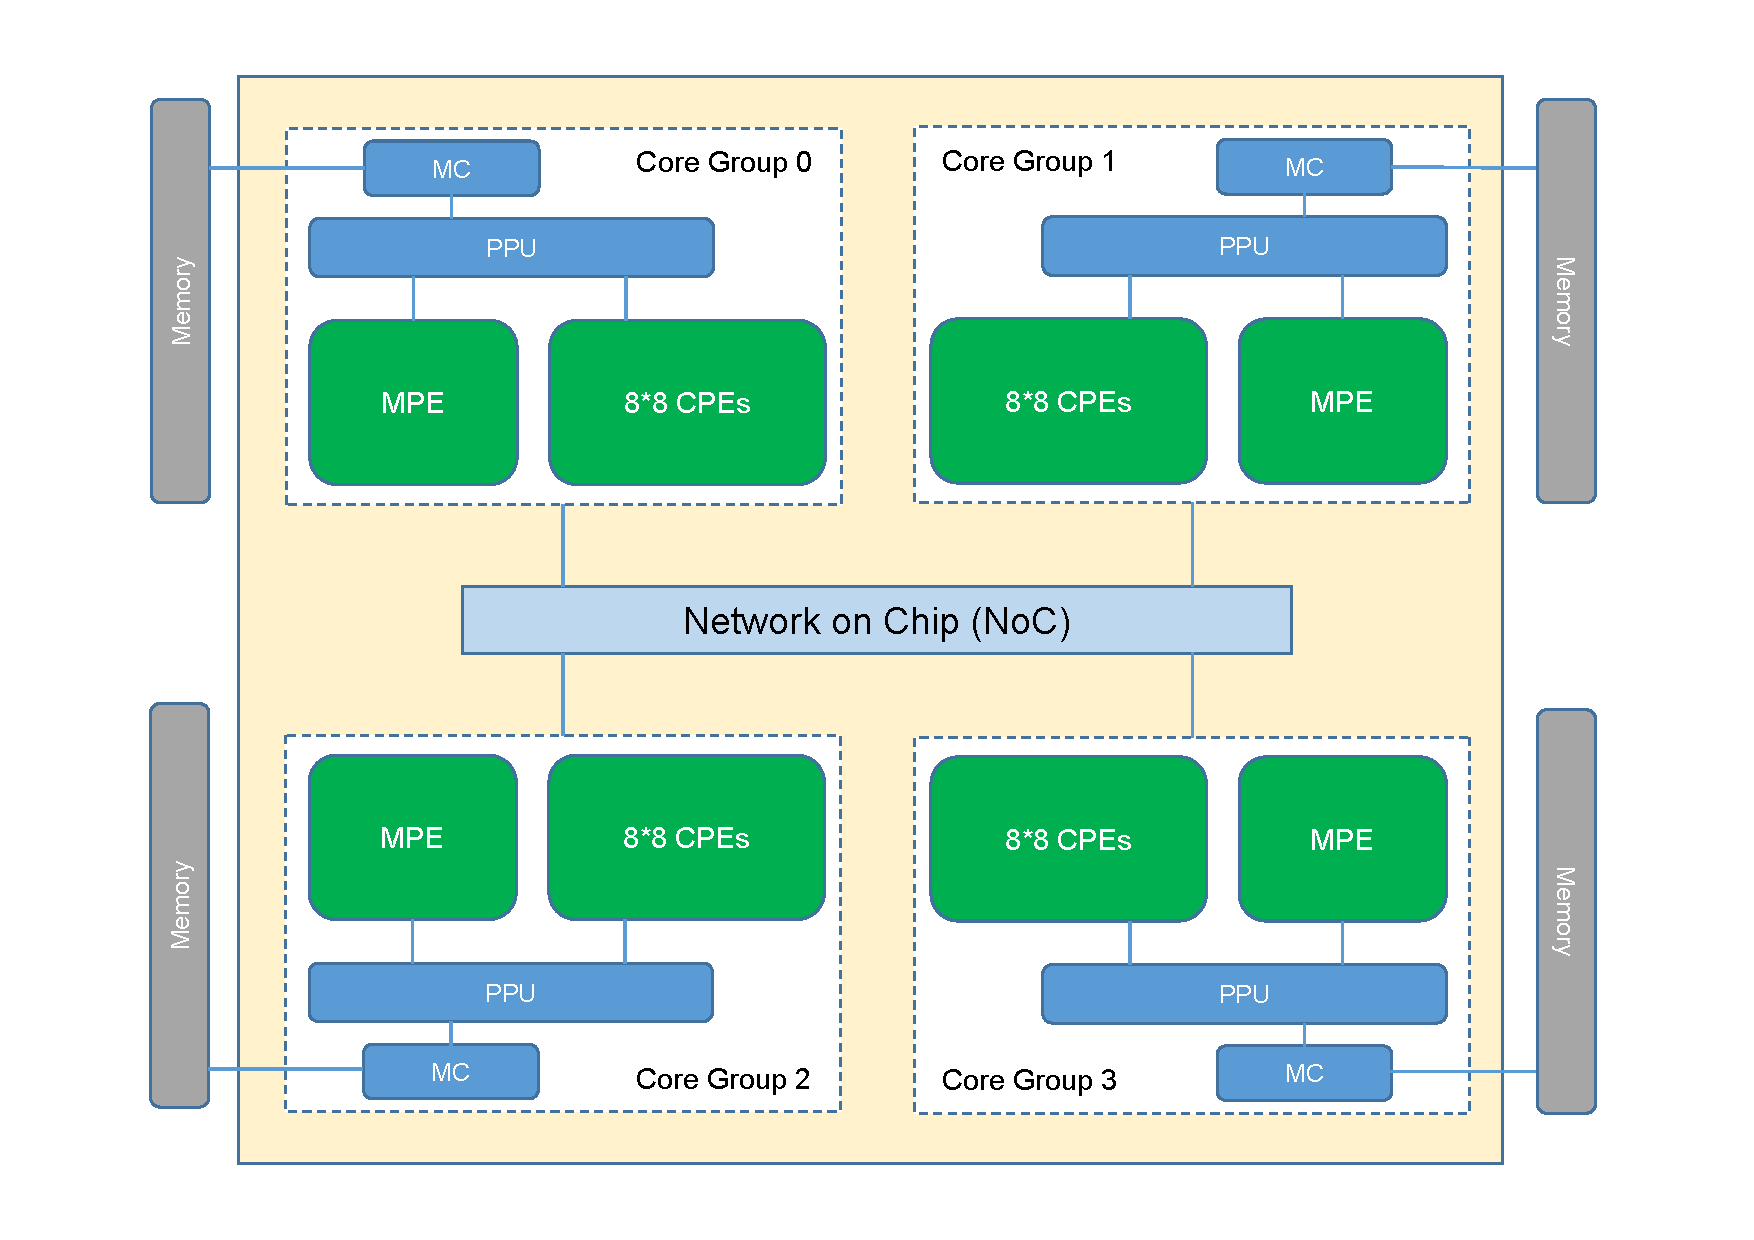
\includegraphics[width=0.45\textwidth]{sw26010.pdf}}
\caption{The architecture of Sunway processor}
\label{sw26010}
\end{figure}
It can provide a peak performance of 3.06 TFlops and a performance-to-power ratio of 10 GFlops/Watt. The processor contains four Core Groups (CGs) and each CG is composed of one Management Processing Element (MPE), one DDR3 Memory Controller (MC) and one Computing Processing Elements (CPEs) cluster with 64 CPEs organized as 8 by 8 mesh. Each CG has 765 GFlops double-precision peak performance and 34.1 GB/s theoretical peak memory bandwidth. The MPE targeting at task management is a complete 64-bit RISC core with a frequency of 1.45 GHz, supporting complete interrupt functions and out-of-order execution. In contrast, CPE is a simplified 64-bit RISC core to maximize the aggregated computing power and CPEs in one CG share 4 memory channels.

As for the memory hierarchy, each CG connects to its own 8GB DDR3 memory accessed through Direct Memory Access (DMA) for the MPE and CPEs. The Network on Chip manage the memory of four CGs and the size of each CG's private memory space can be customized by users. The MPE has a 32KB L1 instruction cache, a 32KB L1 data cache and a 256KB L2 cache for both instruction and data, while each CPE provides a 16KB instruction cache and a 64KB Local Device Memory (LDM). The programmable LDM is controlled by users through software. The processor provides an important data sharing capability across the CPEs: register communication, which enables the CPEs in the same row or column communicate with each other with ten clock cycles. A performance model based on the three-level (REG-LDM-MEM) memory hierarchy was proposed \cite{b16}.

Sunway architecture provides two parallel programming models, "MPI+OpenACC" or "MPI+Athread". In most cases, each CG corresponds to one MPI process and OpenACC or Athread are adopted to exploit the performance of 64 CPEs within each CG. As an easy-to-use interface, OpenACC can only perform limited optimization. In contrast, Athread interface supports a number of performance-related programming interface (vectorization, register communication, etc.) to fully exploit the performance potential of SW26010 with enough programming knowledge and efforts. In this work, we adopt the Athread programming interface with careful algorithmic adjustment into consideration.

\subsection{Multi-Level Blocks strategy}

As mentioned above, the computational capability in unstructured mesh is limited severely by the indirect and irregular addressing. Therefore, we propose Multi-Level Blocks (MLB) method and design a MPE-CPEs asynchronous parallel algorithm. Fig. \ref{mlb(overview)} presents the decomposition of an unstructured mesh and its matrix form with LDU format.
\begin{figure}[tbp]
\centerline{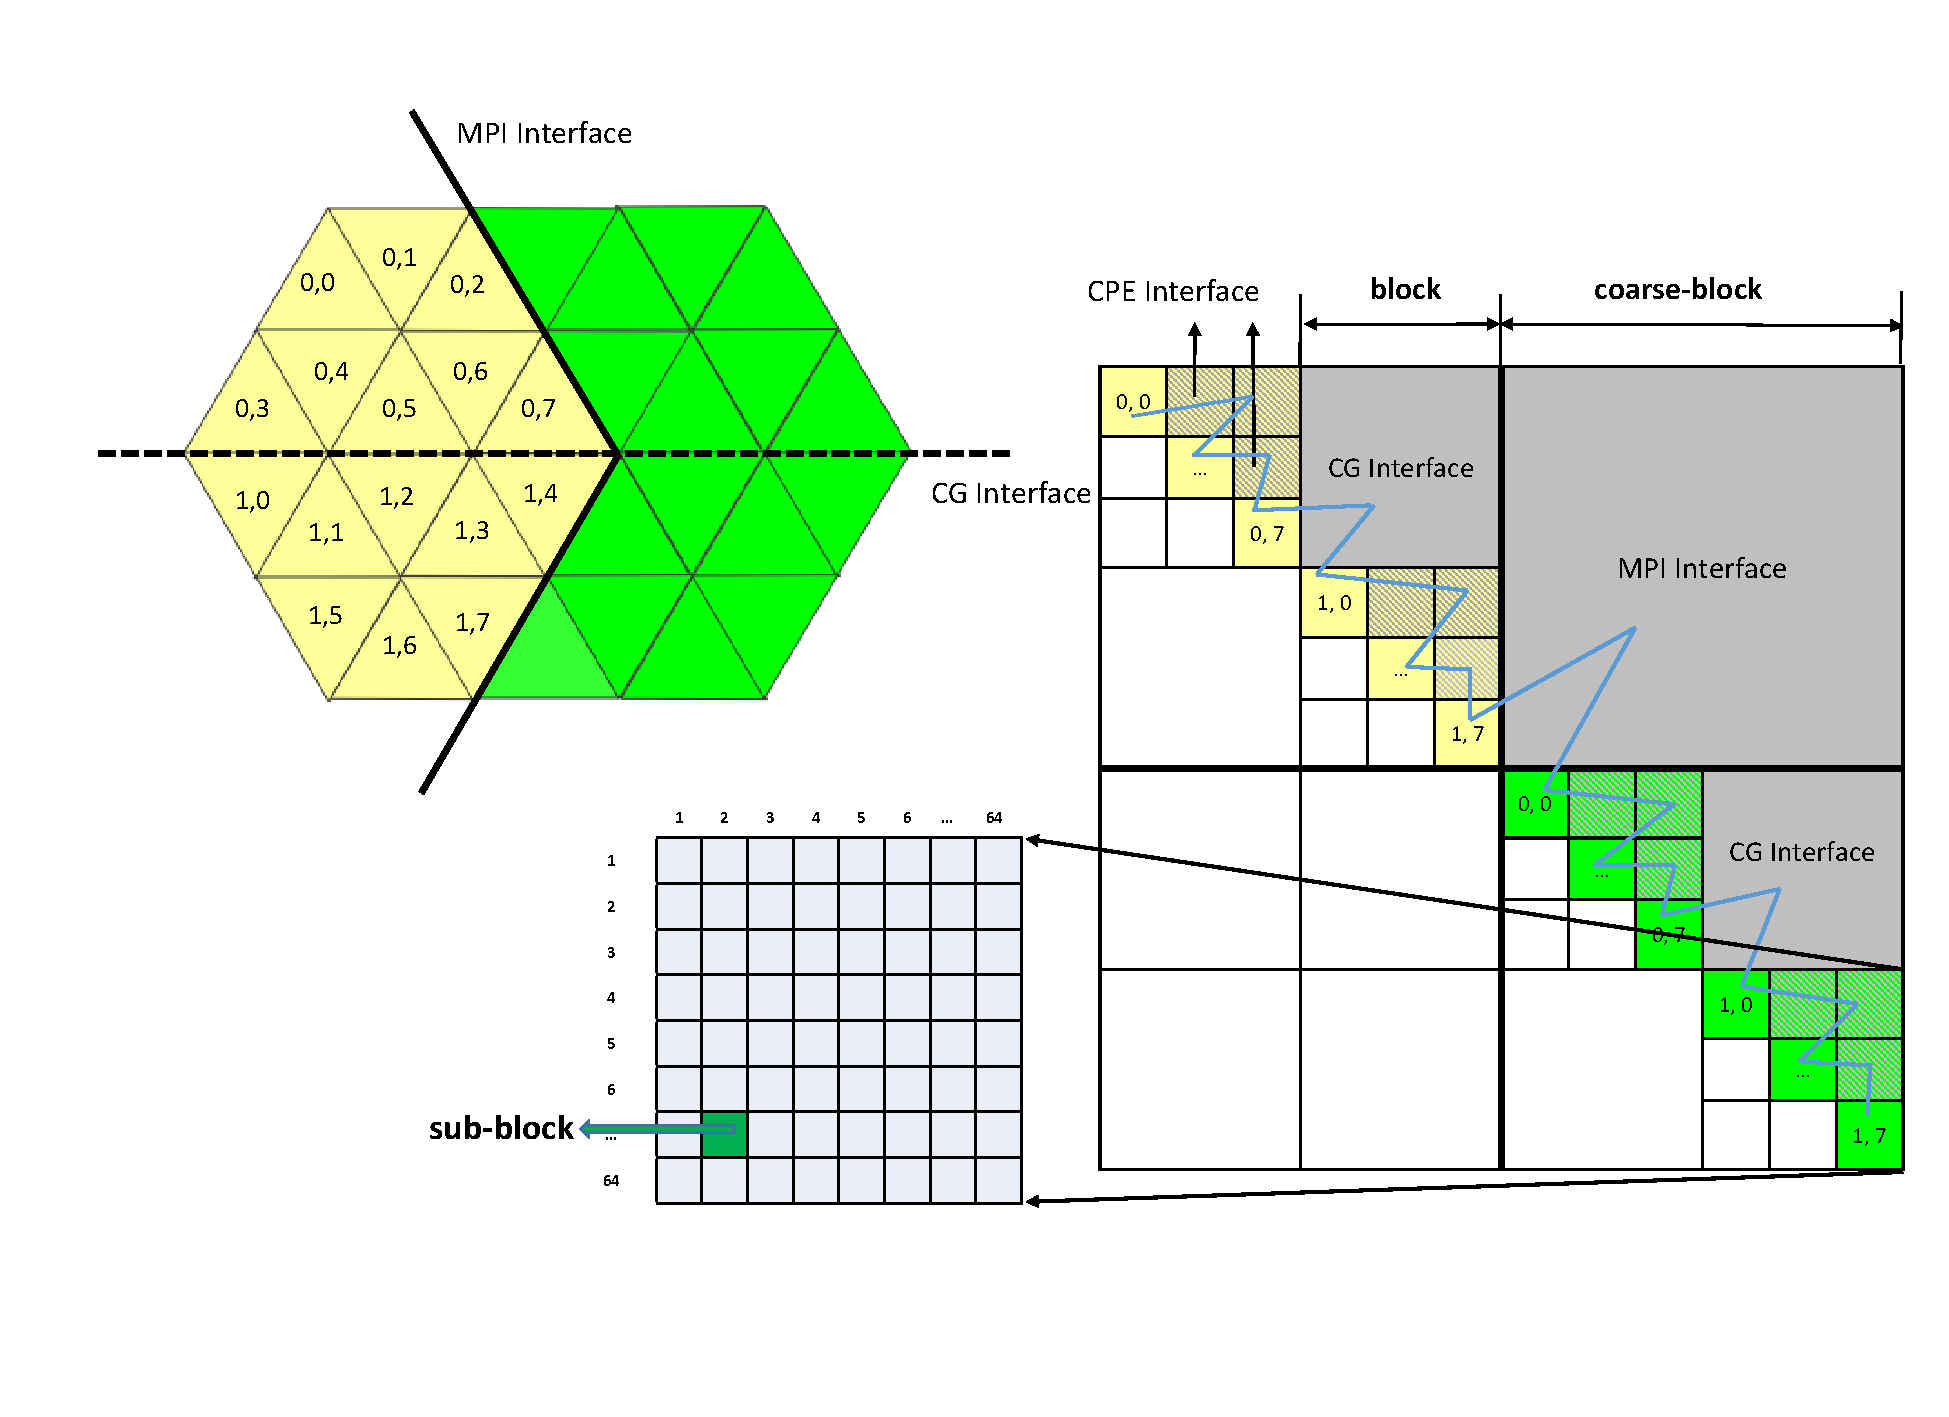
\includegraphics[width=0.45\textwidth]{mlb(overview).pdf}}
\caption{Multi-Level Blocks of unstructured mesh. The unstructured mesh is decomposed and assigned to two processes, colored with yellow and green respectively. Three levels are connected by three interfaces: MPI interface, CG interface and CPEs interface.}
\label{mlb(overview)}
\end{figure}
The data structure in MLB is a non-uniform multi-block structure. The coarsest block ($coarse-block$) represents the mesh decomposition at MPI level. The non-zeros on diagonal $coarse-block$ represent the internal faces of mesh cells inside one process assigned to a single CG, and the off-diagonal $coarse-block$ is the MPI interface between associated processes. The medium block ($block$) is partitioned according to the limitation of LDM size and then the whole relevant data of $blocks$ can be stored in LDM thoroughly. At this level, all $blocks$ are categorized as internal blocks (marked as colored cells in the diagonal $block$) and CG interface blocks (marked as gray cells in the off-diagonal $block$), assigned to CPEs and MPE respectively with the data density into consideration. This pattern will introduce a read-write conflict between MPE and CPE if they are in charge of the same row. The issue can be eliminated through adding a bias to the row indices of blocks in MPE relative to CPEs.

Finally, the finest block ($sub$-$block$) is decomposed based on the hardware of CG. The number of $sub$-$block$ is set to a fixed value, 64, corresponding to the amount of CPEs in one CG. The diagonal $sub$-$block$ is "local" for the corresponding CPE and the off-diagonal $sub$-$block$ is the CPE interface. The "local" data is loaded into LDM by DMA directly while the data in the interface is transferred by on-chip register communication because of the discreteness and sparsity. The blue filling curve in Fig. \ref{mlb(overview)} indicates the storage sequence of different blocks in memory. Generally, the priority rule is that the finer level block is prior to coarser ones and in the same level row block is prior to column block. Inside the $sub$-$blocks$, the edge sequence is arbitrary. Taking advantage of the graph partition tool Metis, most face can be gathered in diagonal blocks for each level and interfaces can be minimized to a certain extent with load balance into consideration. 

So far we obtain a block-structured and organized data structure through MLB. The off-diagonal $block$, CG interfaces, are in the charge of MPE and the computation process is nearly identical to serial code. As for the computation of diagonal $block$ in CPEs, one CPE is in charge of the $sub$-$blocks$ in the same row. To explain the computational pattern of CPEs, we take SpMV as example. The coefficient matrix $A$ with LDU format is decomposed as three arrays, $lower$, $upper$ and $diag$, storing the lower triangle, upper triangle and diagonal data respectively. These data can be loaded into LDM through DMA because of its consecutiveness in memory, while this pattern is not appropriate to vector $x$ and $b$. The computation process of diagonal $block$ in CPEs is presented in Fig. \ref{rlc} and the amount of CPEs is cut down to 4 for conciseness.
\begin{figure}[tbp]
\centerline{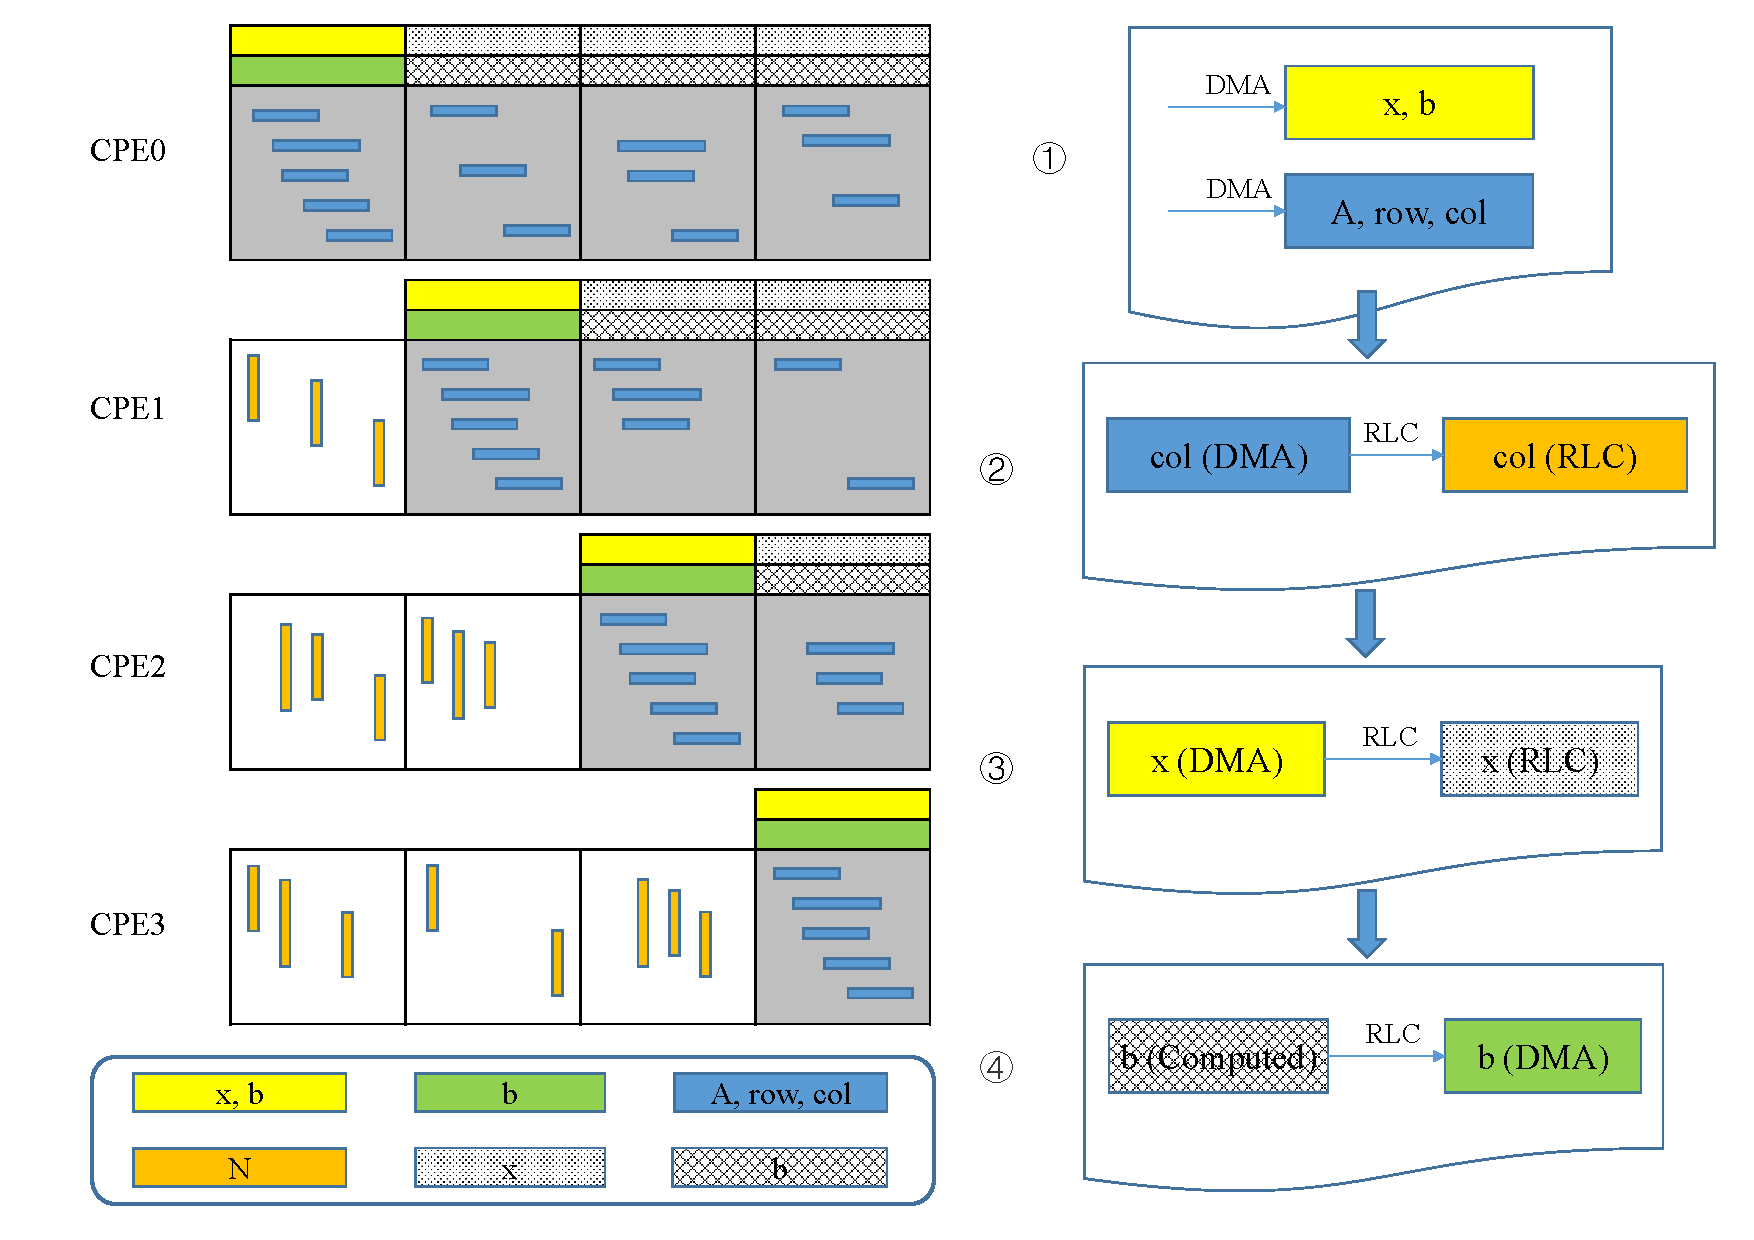
\includegraphics[width=0.48\textwidth]{rlc.pdf}}
\caption{The computation process in CPEs: (1).Fetch "local" $x$, $b$, $A$ and the connectivity $row$ and $col$ through DMA; (2).Get $col$ in the lower triangle from other CPEs through Register-Level Communication (RLC); (3).Scatter the diagonal $x$ to other CPEs through RLC; (4).Gather the off-diagonal $b$ from other CPEs through RLC.}
\label{rlc}
\end{figure}
In our implementation, the data of the diagonal $sub-block$ and off-diagonal $sub-blocks$ are considered as "local" data and "global" data respectively. Firstly, the non-zeros of adjacency matrix $A$ and the connectivity (row indices $row$ and column indices $col$) are loaded into LDM through DMA with local $x$ and $b$ (\textcircled{1}). Then we transfer the column indices $col$ from the upper triangle to the lower triangle through Register-Level Communication (RLC), which is essential for the next step (\textcircled{2}). The global $x$ cannot be loaded directly through DMA because of the redundancy of $x$ and the limited LDM space, while it is stored in the LDM of other CPEs. Hence $x$ can be selected corresponding to the column indices $col$, and scattered to other CPEs. Then we can obtain the "sparse" global $x$ for each CPE, the same layout as $A$ (\textcircled{3}). Now that the adjacency matrix $A$ and vector $x$ are loaded into LDM, we can perform SpMV operation on the CPEs and get the output vector $b$ with the same storage layout as $x$. To avoid the write conflict between CPEs, $b$ needs to be gathered to the corresponding CPEs through RLC, which can be noted as "owner-write" model (\textcircled{4}).

As mentioned above, the unstructured mesh is decomposed into three levels in MLB method. The counts of coarsest blocks and finest blocks are determined by the main memory of CGs and the number of CPEs of CGs respectively. For the medium blocks, the count $N$ is estimated according to the LDM size by the following equation:
\begin{equation}
\begin{aligned}
    N&=\frac{\sum_{1}^{n}(C_{i}*L_{i}*D{i})\times sizeof(swFloat)}{CPE_{num}\times size_{ldm}} \\ 
    &+\frac{2\times N_{con}\times sizeof(swInt)}{CPE_{num}\times size_{ldm}}
\end{aligned}
\end{equation}
$C_{i}$, $L_{i}$ and $D_{i}$ are the array number defined on the data sets, the length of arrays and the dimension of arrays, corresponding to the three levels of SoAoS structure. Normally the value of $n$ is equal to 2, which indicates there are two data sets such as face and cell in FVM method or node and edge in FEM method. $swFloat$ and $swInt$ are our alias of float and integer for the convenience of type definition in UNAT. $N_{con}$ is the length of connectivity arrays, $row$ and $col$ in SpMV. $CPE_{num}$ and $size_{ldm}$ are the amount of CPEs in one CG and the size of LDM space, 64 and 64KB respectively.

\subsection{Row-Subsections strategy}

The accurate data tiling is the critical strategy in this implementation. In an adjacency matrix, rows and non-zeros are decomposed sequentially in two levels as shown in Fig. \ref{rss(overview)}. The first level contains 64 segments, consisting of the number of CPEs in a CG, and the second level is determined according to the LDM capacity of a single CPE. This is a light weight algorithm without any adjustment to the original topology. $row$ in the name $Row-subsection$ indicates that rows are the fundamental unit for decomposition and the name $subsections$ indicates a number of subsections, generated by tiling the non-zeros data sets. In a matrix view the subsections are the projections of non-zeros to the column, marked as $Column Subsections$ in Fig. \ref{rss(overview)}. Take SpMV as example, the column related data sets, $x$ and $b$, are organized as multiple contiguous subsections, and then we can perform effective and consecutive memory access.
\begin{figure}[tbp]
	\centerline{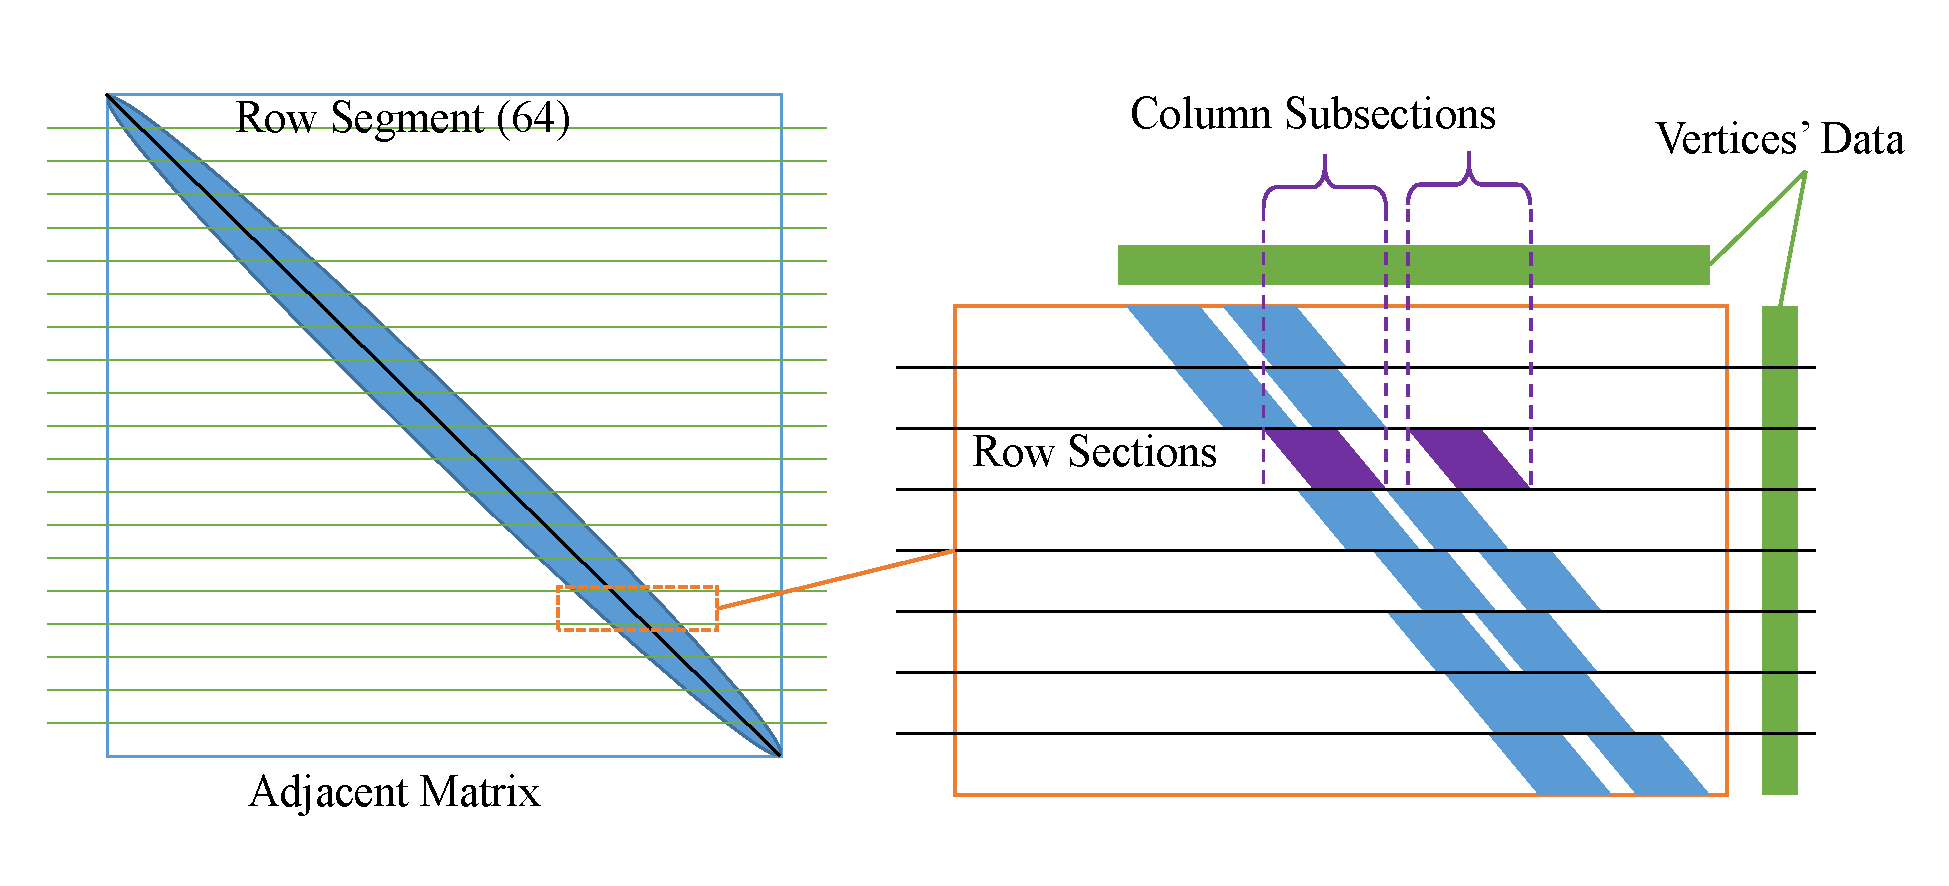
\includegraphics[width=0.48\textwidth]{rss(overview).pdf}}
	\caption{Two level decomposition and the projection of column subsections in RSS strategy. The blue region along the diagonal line (black) of the adjacency matrix (left) is where the entries are located. One row segment is scaled up at the right part, where the scattered diamond blocks (blue and purple) represent that the non-zeros can be placed into one column subsections. The purple notations showed the projecting of column related data sets on vertices (green bars).}
	\label{rss(overview)}
\end{figure}

Different from OP2\cite{b2}, the counts of subsections for each row section is variable and the span of the subsections is adaptive in different application situations. A multiple-nearest algorithm is adopted in the column subsections projection. In the algorithm, the non-zeros are traversed in a row-first sequence, and the given span determines whether the column of non-zeros should be put into a previous subsection or start a new subsection. The span is critical for performance tuning, since small span will cause fragmented subsections and low memory bandwidth, while large span may involve too many redundant data and thus reduces the effective bandwidth. We prepare a mini program to measure the DMA bandwidth under various sizes of data block and the results are presented in Tab. \ref{bandwidth}.
\begin{table}[]
\centering
\caption{DMA Bandwidth between global memory and LDM}
\label{bandwidth}
\begin{tabular}{cc}
\hline
Size(Byte) & DMA Bandwidth(GB/s) \\ \hline
8          & 0.97                \\
32         & 4.82                \\
64         & 12.84               \\
128        & 18.46               \\
512        & 23.27               \\
1024       & 28.71               \\
2048       & 29.53               \\
4096       & 31.56               \\ \hline
\end{tabular}
\end{table}
It is clear that the bandwidth nearly reach its peak performance when the size of data block exceed 1025 Bytes. Then the initial value of span by the following equation:
\begin{equation}
\label{colLen}
    L=\frac{1024}{sizeof(swFloat))}
\end{equation}
This value will be halved if there are too many redundant data in subsections and this process will be performed repeatedly until the sum of spans is greater than the counts of non-zeros in the overall subsections. Minimum bandwidth rearrangement is required on some occasions to improve the quality of matrix, which is also provided in UNAT API.

An important problem of the RSS strategy is the race condition between CPEs under LDU format. We design a coloring algorithm to address the write conflicting problem. As shown in Fig. \ref{rss_color},
\begin{figure}[tbp]
	\centerline{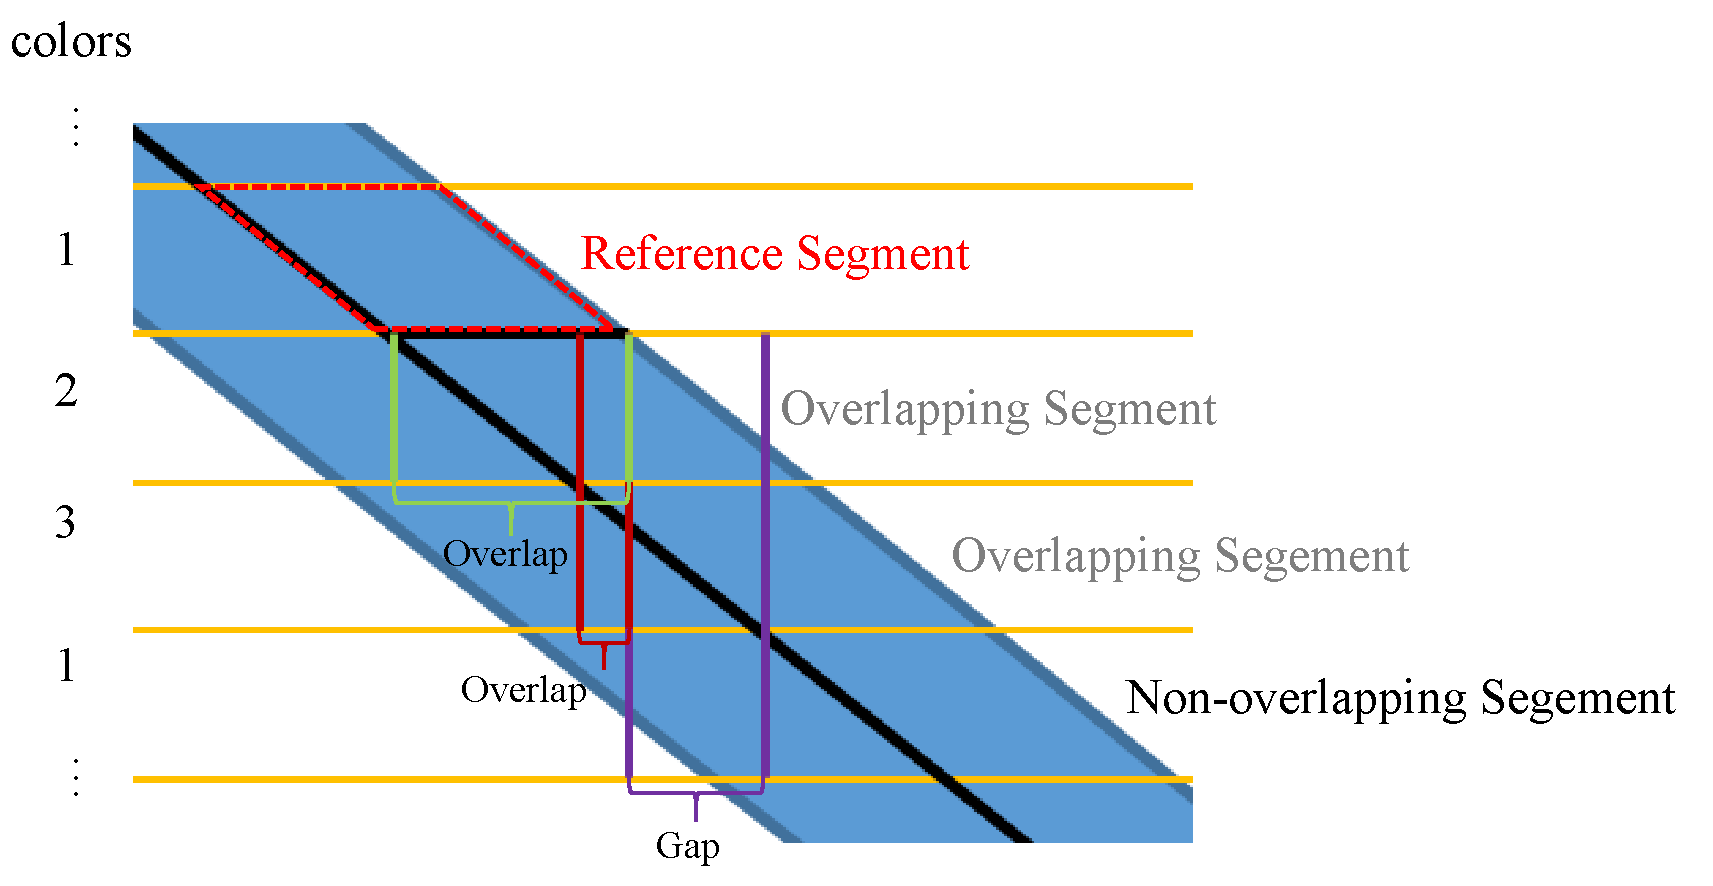
\includegraphics[width=0.48\textwidth]{rss_color.pdf}}
	\caption{The RSS segment coloring. Only upper triangle matrix (blue region upon the black line) is considered because of the symmetric format. The reference segment is boxed with red dash lines. Overlapping Segments are labeled with grey words and non-overlapping segments with black ones. The round of write operation are label to the left of each segment.}
	\label{rss_color}
\end{figure}
 typical adjacency matrix can be reordered with limited bandwidth, so the non-zeros of referenced row segment will not overlap with the subsequent segments when the distance between them are large enough. Following this method, the algorithm colors non-overlapping segments as many as possible into a single class to ensure the maximal concurrency of write operations. To our experience, a representative adjacency matrix of real-world application will often have a bandwidth smaller than 1/10 of the matrix’s rank, so there will be on average more than 10 concurrent threads for each colored class, far enough to utilize the 4 memory tunnels for CPEs in a CG. The coloring algorithms commonly have an $O(logN)$ complexity, and in this work N is always 64 since the coloring is performed on segments whose number is constantly 64 equalling to the amount of CPEs in a single CG. So the RSS strategy is still very light-weight.
 
 \section{Performance}
 \label{sec:perf}

\subsection{Experiment Setup}
In this section, quantitative experiment results are presented and discussed to evaluate the performance of UNAT. We select Sparse Matrix-vector Multiply (SpMV) as the measured operator. SpMV plays an important role in linear algebra algorithms, which is well adopted for computational fluid dynamics (CFD), molecular dynamics (MD), and some machine learning algorithms such as convolution neural network (CNN) deeply rely on SpMV. However, SpMV is not friendly for many-core architectures because of the irregular memory access and write conflicts \cite{b8}, which is appropriate to examine the efficiency of UNAT. As is mentioned above, we separate the specification of a computational operator with its parallel iteration details. Hence the specification of SpMV in UNAT is roughly identical to its implementation in the serial edition as shown in Fig. \ref{spmv}.

We perform various experiments to reveal the performance of UNAT thoroughly and the details are presented in Tab. \ref{expDetail}. Iterator with MLB and RSS strategies mentioned above are the main performance objectives and we will illustrate the results in the next sections respectively. We select two types of matrices and two representative sparse matrices format, LDU and COO. The matrix applied to MLB strategy is the boxTube16 case from the tutorials of OpenFOAM, which performs DNS with the finite volume scheme. The other one applied to RSS strategy is from the University of SuitSparse Matrix Collection \cite{b9}, and it is used to solve Navier-Stokes and similar transport equations with finite element discretization. Both of them have series of matrices with similar topology and different non-zeros, ranging from 30K to 700K. Moreover, to compare performance of UNAT across SoA and AoS data layout, we set four different numbers of components, $N$, in struct and the values are corresponding to the variable types scalar, vector, symmetric matrix and asymmetric matrix respectively. The data layout naturally transforms from AoS to SoA when the number of components equals to 1.

% Please add the following required packages to your document preamble:
% \usepackage{multirow}
\begin{table}[]
\centering
\caption{The specifications of experiments}
\begin{tabular}{|c|c|c|c|c|}
\hline
\textbf{Iterator}             & \textbf{Format}       & \textbf{Matrices}     & \textbf{Rank} & \textbf{Non-zeros}                          \\ \hline
\multirow{8}{*}{MLB} & \multirow{4}{*}{LDU}                       & \multirow{8}{*}{boxTube16} & 10K & 49.6K \\  \cline{4-5}
                     &                                             &             & 20K &119.2K                         \\ \cline{4-5}
                     &                                             &             & 50K &328K                         \\ \cline{4-5}
                     &                                             &             & 125K &860K                         \\ \cline{2-2} \cline{4-5}
                     & \multirow{4}{*}{COO}                        &             & 216K &1.5M                         \\ \cline{4-5}
                     &                                             &             & 300K &2M                         \\ \cline{4-5}
                     &                                             &             & 500K &3.5M                         \\ \cline{4-5}
                     &                                             &             & 100K &6.9M                         \\ \hline
\multirow{10}{*}{RSS} & \multirow{5}{*}{LDU}                        & \multirow{10}{*}{Goodwin}   &10K & 32.3K          \\ \cline{4-5}
                     &                                             &             & 13K &56K                         \\ \cline{4-5}
                     &                                             &             & 17K &98K                         \\ \cline{4-5}
                     &                                             &             & 23K &182K                         \\ \cline{4-5}
                     &                      &                         &
                     30K &312K                         \\ \cline{2-2} \cline{4-5}
                     & \multirow{5}{*}{COO}                        &             & 40K &561K                         \\ \cline{4-5}
                     &                                             &             & 54K &1M                         \\ \cline{4-5}
                     &                                             &             & 71K &1.8M                         \\ \cline{4-5}
                     &                                             &             & 95K &3.2M                         \\ \cline{4-5}
                     &                      &                         &
                     127K &5.8M                         \\ \hline
\end{tabular}
\label{expDetail}
\end{table}

Our experiments are conducted on one CG of Sunway SW26010 processor. The performance of SpMV on a CG is critical because scientific applications on Sunway TaihuLight will generally adopt two-level parallelism and perform the compute-intensive problem, such as SpMV, within CG. We use the application on MPE as our baseline for the performance comparison. All experiments are performed for five times and report the average results in double-precision floating-point arithmetic.

\subsection{Results of Multi-Level Blocks strategy}

In this section, we select boxTurb16 case as the generator of sparse matrix and we obtain eight representative scales of matrices through adjusting the number of cells in every dimension.
The performance of MLB method with LDU format is presented in Fig. \ref{mlbldu}. 
\begin{figure}[tbp]
\centerline{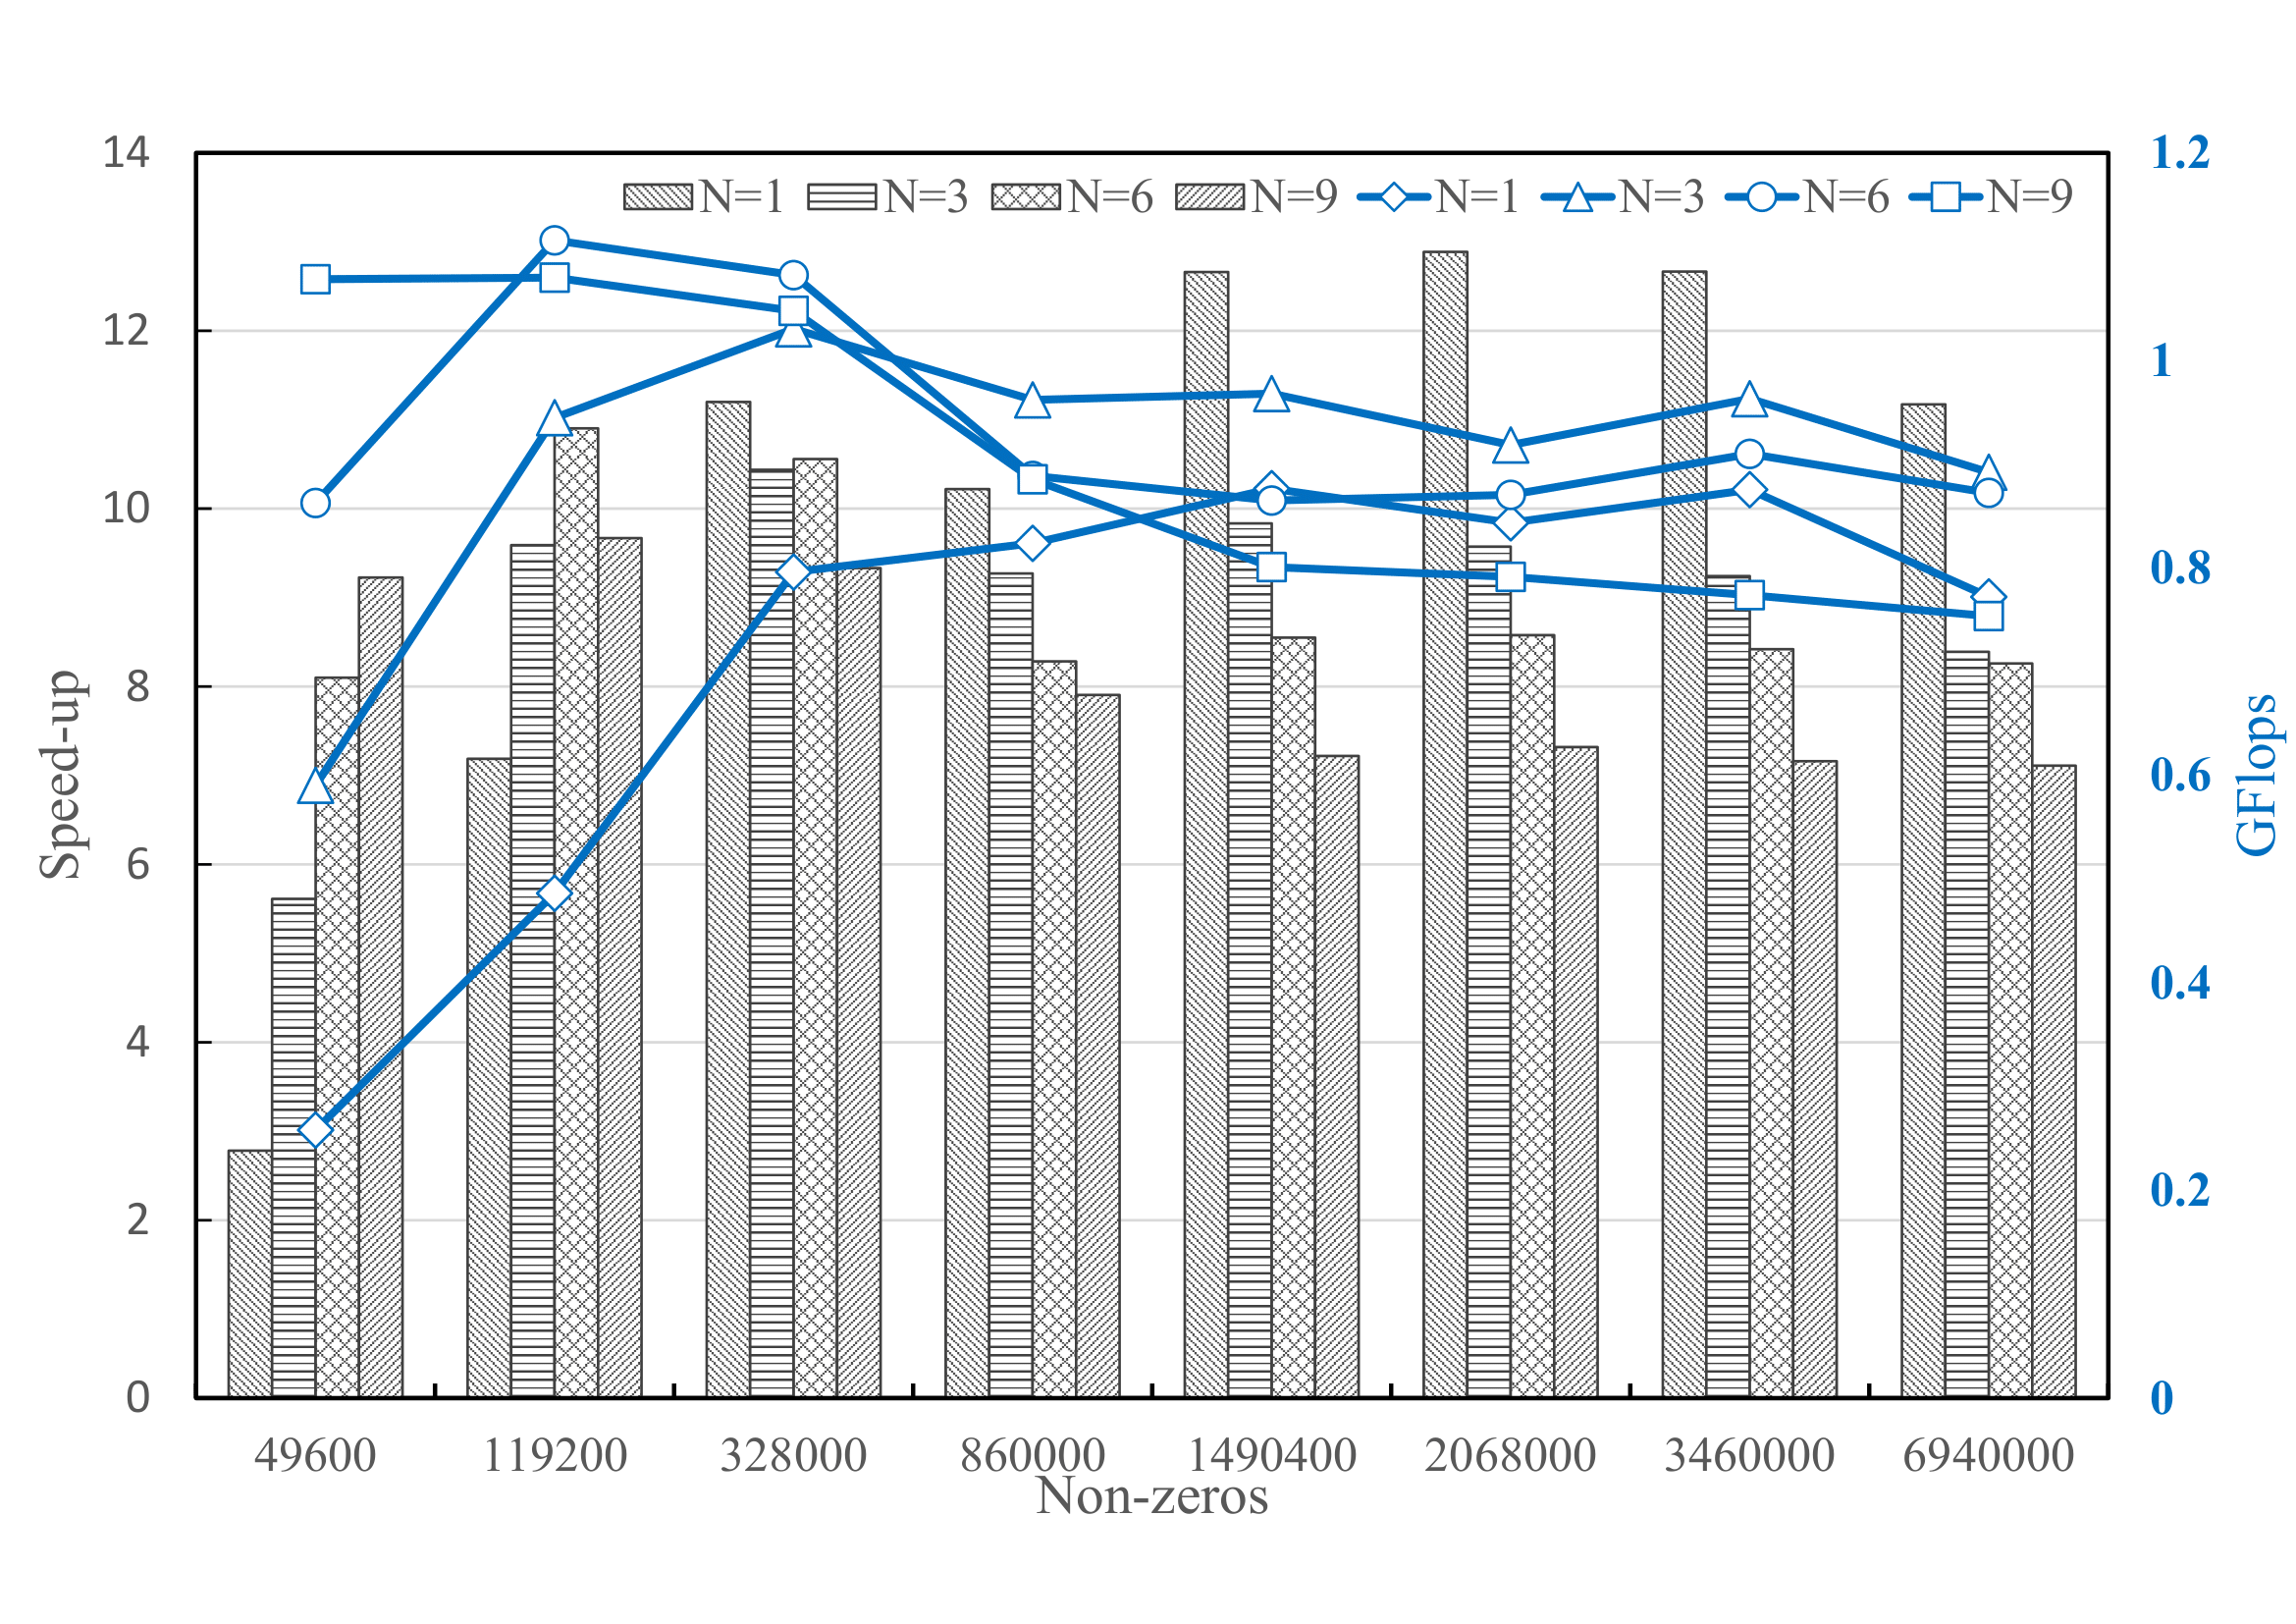
\includegraphics[width=0.45\textwidth]{mlb(ldu)-1.png}}
\caption{The speed-up of MLB iterator with LDU format compared to the baseline. $N$ indicates the number of components in the struct. Bar graph: left y-axis. Line graph: right y-axis.}
\label{mlbldu}
\end{figure}
The speed-up of MLB method slightly increases with the number of non-zeros and reaches its best performance at around 2 million entries. The reported speed-up is 12 on an average when $N=1$ while about 70 percent of performance can be obtained under other circumstance. The reason can be summarized as three factors.

Firstly, the AoS storage pattern is not friendly to many-core architectures because of the stride between different components \cite{b10}\cite{b11}. Secondly, the topology of RLC is only determined by the topology of matrix and independent of the data layout for the compatibility, so the RLC will be performed $N$ times serially, which equals to number of components. Finally, within the limited LDM space, the number of blocks has a variation of direct proportion with the number of components while the non-zeros assigned to one CPE takes the reverse direction. The increase of proportion of off-diagonal blocks indicates the increase of communication boundary among CPEs, which gives severe pressure to the RLC.

However, we can not conclude from the speed-ups that we can get better performance from SoA storage pattern than AoS for MLB iterator. The speed-ups only reveal the performance of one of the components in SoA while these components are managed in the outer loop serially. A more precise measurement about the performance of SoA and AoS is the Floating-point operations per second (Flops), which is also presented in Fig. \ref{mlbldu}. The Flops of AoS is slightly higher than that of SoA except for $N=9$ when the matrix size is large enough, and for the smallest matrix the Flops of $N=9$ is the highest. This implies that SoA storage pattern is the better choice for MLB strategy in view of the performance, which can also be demonstrated in Fig. \ref{mlbcsr}.

On the other hand, Fig. \ref{mlbcsr} illustrates the performance of MLB method with COO format.
\begin{figure}[tbp]
\centerline{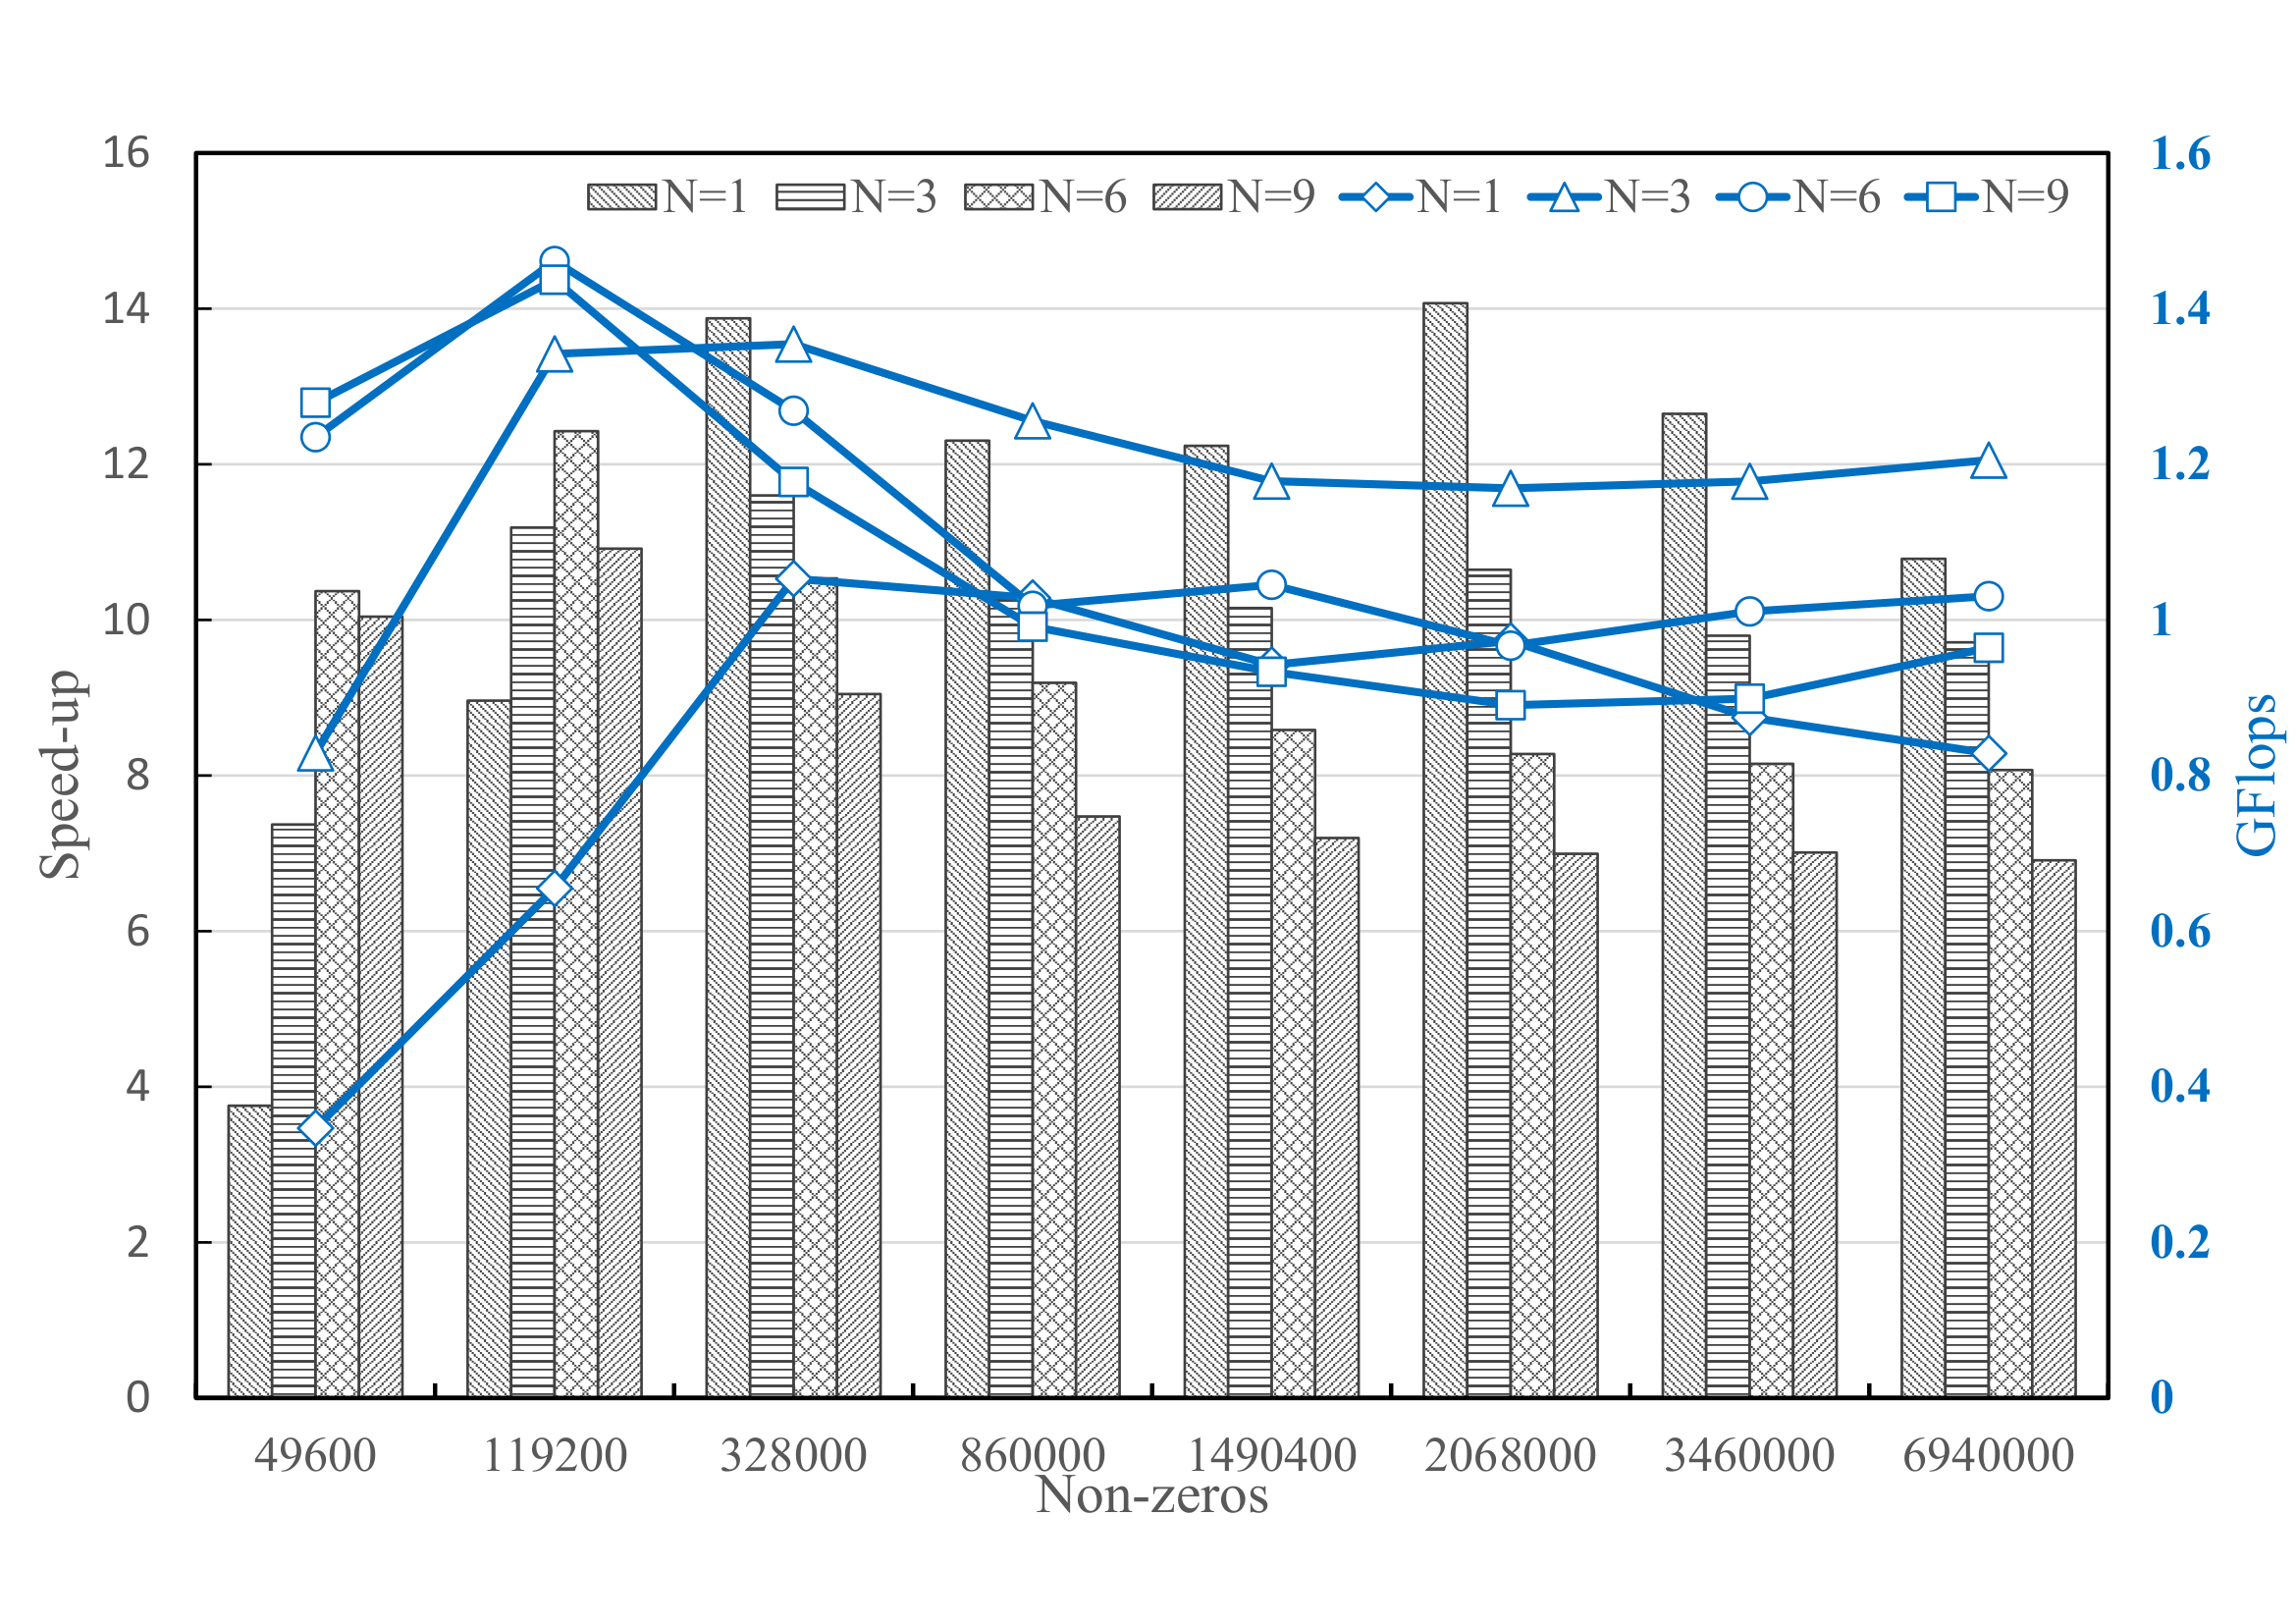
\includegraphics[width=0.45\textwidth]{mlb(csr)-1.png}}
\caption{The speed-up of MLB method with COO format compared to the baseline. $N$ indicates the number of components in struct. Bar graph: left y-axis. Line graph: right y-axis.}
\label{mlbcsr}
\end{figure}
The trend with respect to AoS and SoA is similar to LDU, but it is obvious that we obtain 10$\sim$20 percent performance gain from COO format whether AoS or SoA. The main advantage of COO format is the absence of write conflicts. For LDU format, RLC will be performed twice to transfer global $x$ and $b$, while only global $x$ need to be transfered through RLC for COO format. However, this benefit is at the cost of redundant computations, similar to the "owner-compute" model\cite{b2}, while it is not evident for SpMV because of the existence of lower triangle. In some flux computation of finite volume scheme, the sparse matrix is symmetric structurally and numerically and then the computation of lower triangle is needless. But the cost of redundant computations in COO format is not so evident for Sunway processor benefiting from its higher ratio of computing capacity to memory bandwidth. The performance of these two matrix format for one certain problem has to be measured and analyzed dialectically.

\subsection{Results of Row-Subsections strategy}

In this section, we select ten Goodwin matrices from the University of Suit Sparse Matrix Collection. Goodwin is a finite-element matrix in a nonlinear solver, provided by Ralph Goodwin of the University of Illinois at Urbana-Champaign. The performance of RSS method with LDU format is presented in Fig. \ref{rssldu}.
\begin{figure}[tbp]
\centerline{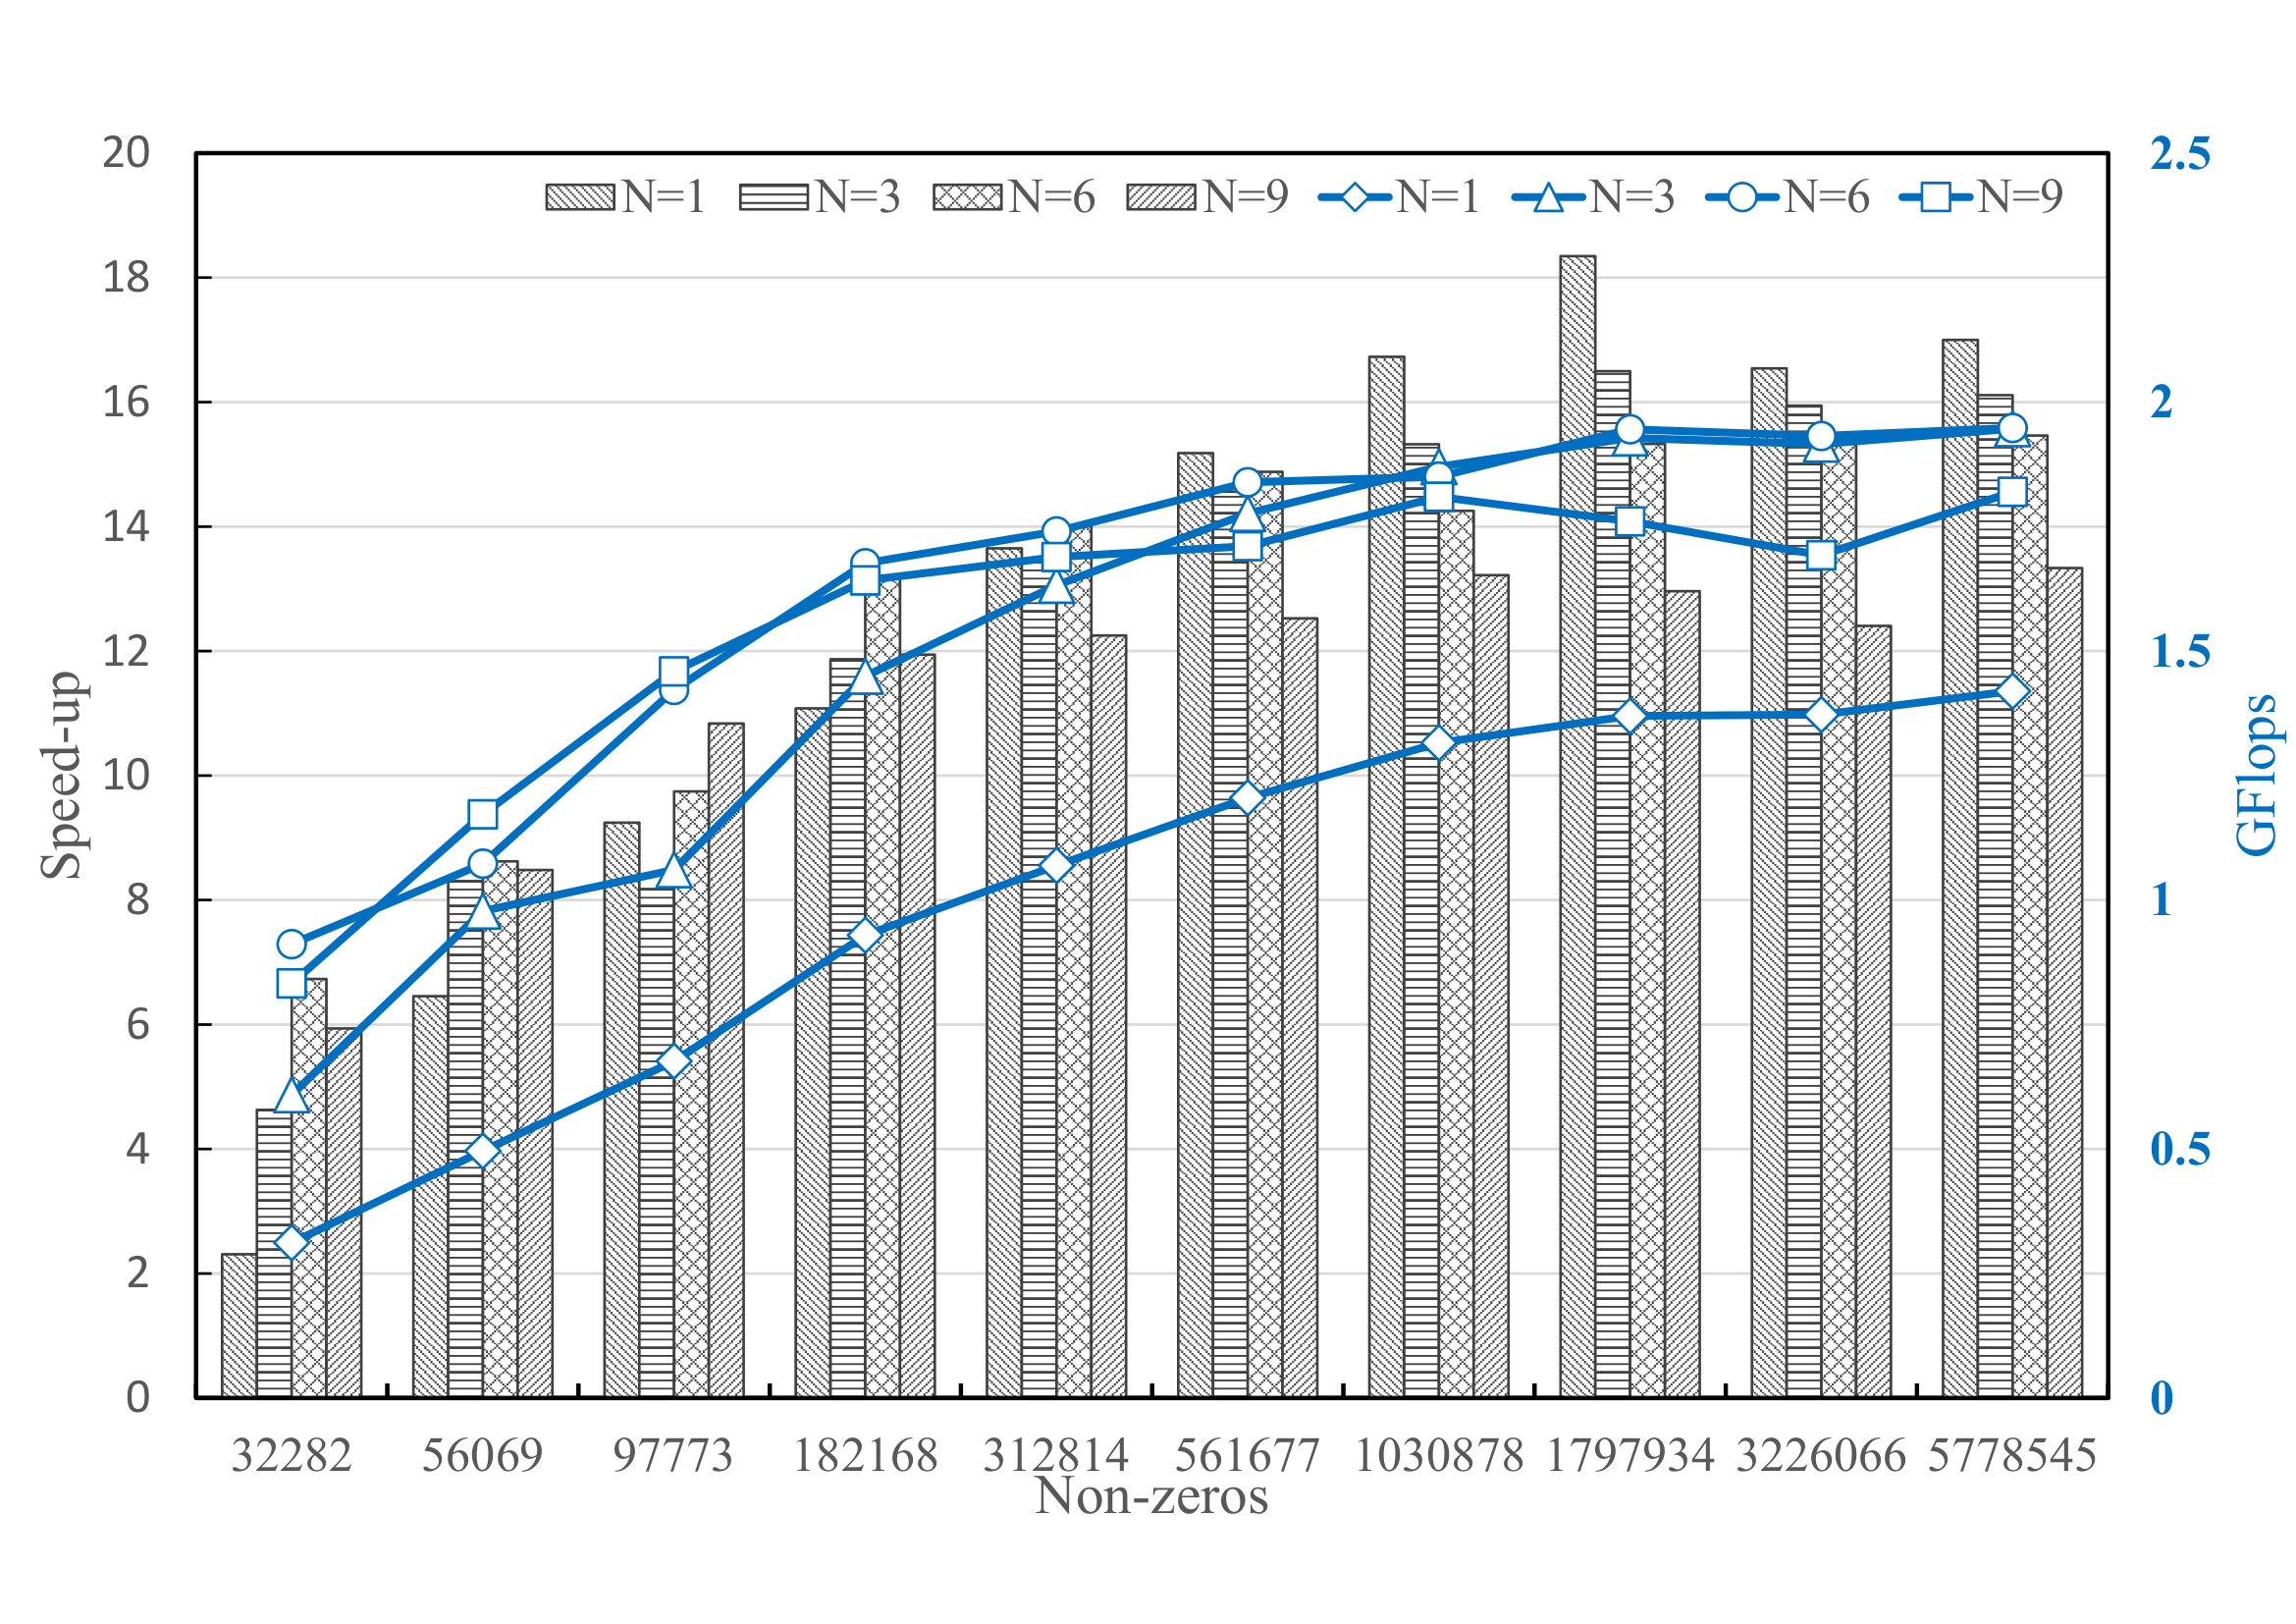
\includegraphics[width=0.45\textwidth]{rss(ldu)-1.png}}
\caption{The speed-up of RSS iterator with LDU format compared to the baseline. $N$ indicates the number of components in struct. Bar graph: left y-axis. Line graph: right y-axis.}
\label{rssldu}
\end{figure}
In general, our implementation achieves 15$\times$ speed-up on average compared to the base line and the Flops reach almost 2 GFlops. The obvious gap between AoS and SoA is primarily caused by the colored write algorithm. For SW26010, the bandwidth of DMA progressively increases and nearly reachs its peak performance when the size of continuous memory access blocks reach 1024 Bytes. Hence the span $L$ of column-subsection is determined by Equation (\ref{colLen}),
Compared to the SoA pattern ($N=1$), AoS pattern has shorter column-subsection, which provides two benefits for DMA: firstly, it reduces the ratio of redundant columns without the bandwidth changed; on the other hand, the shorter column-subsection indicates the less overlap across the CPEs, which reduces the amount of DMA rounds.

Fig. \ref{rsscsr} illustrates the performance of RSS method with COO format.
\begin{figure}[tbp]
\centerline{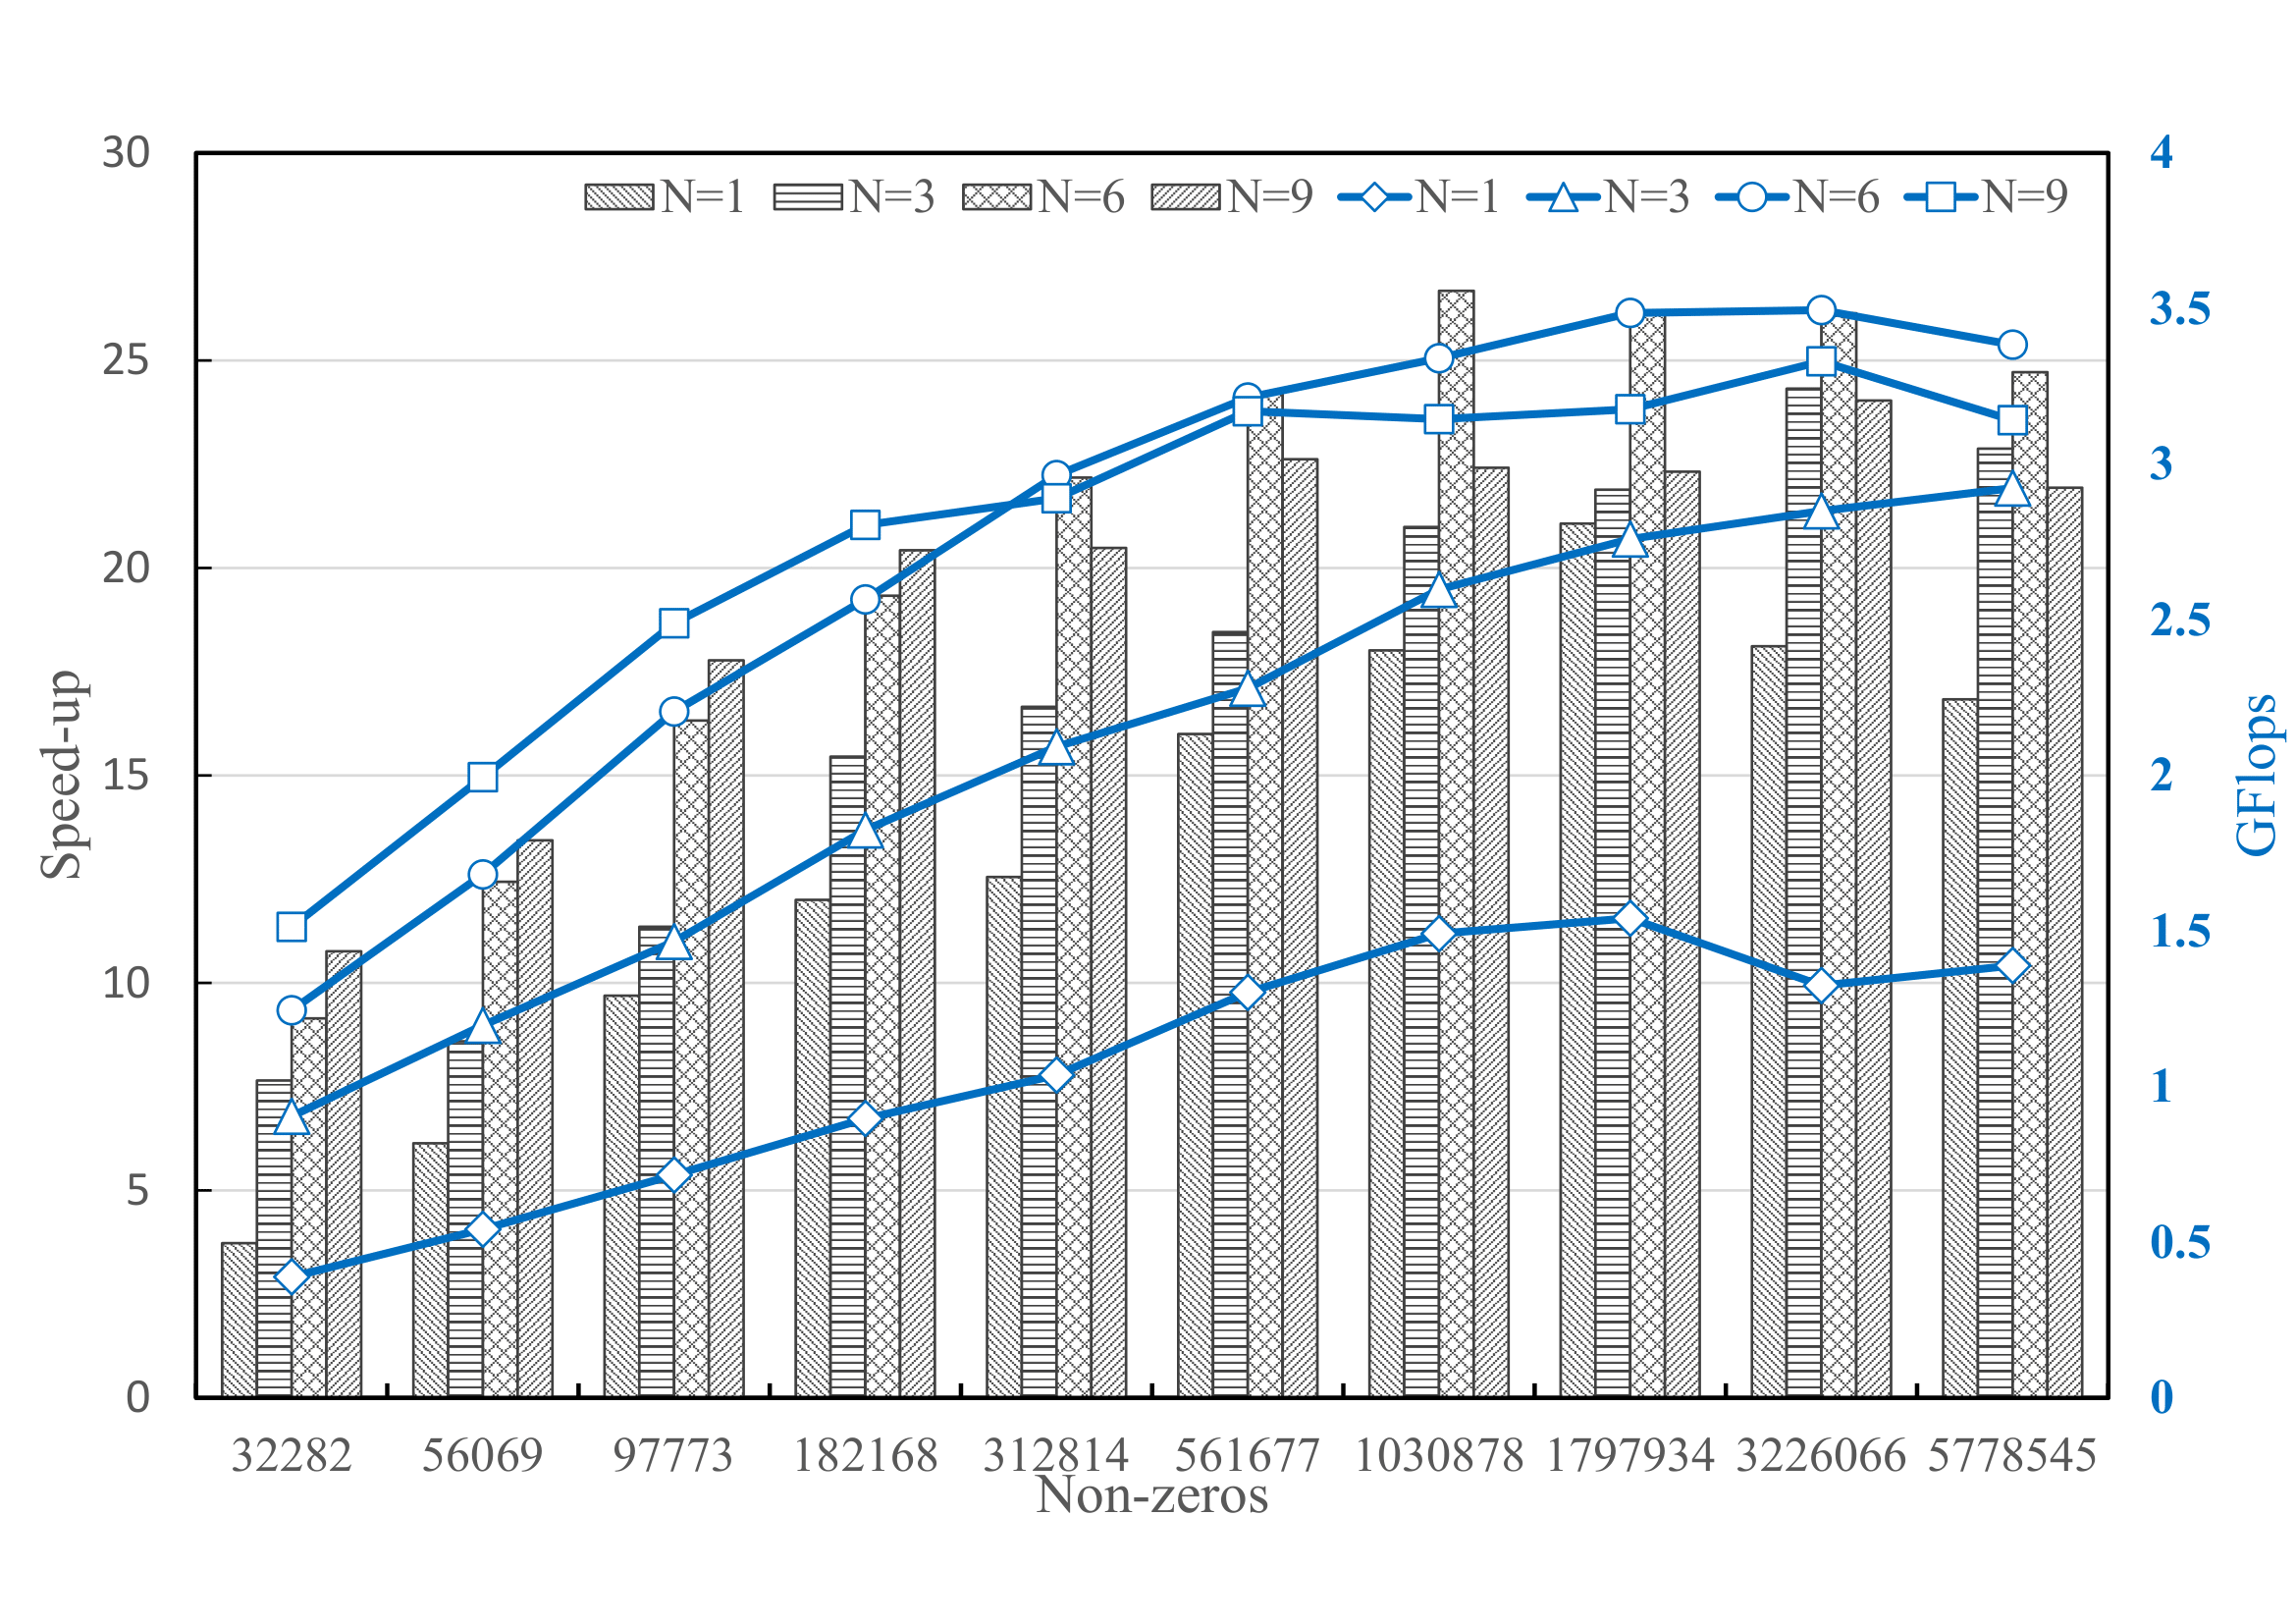
\includegraphics[width=0.45\textwidth]{rss(csr)-1.png}}
\caption{The speed-up of RSS method with COO format compared to the baseline. $N$ indicates the number of components in struct. Bar graph: left y-axis. Line graph: right y-axis.}
\label{rsscsr}
\end{figure}
The highest reported speed-up and Flops reach nearly 27 and 3.5 GFlops respectively and the overall performance of COO pattern is 1.5x compared to LDU pattern. The obvious difference is caused by write conflict, which has been explained in the last section. Similarly, the redundant computation is "meaningful" with the existence of lower triangle in SpMV operator. To illustrate the influence of redundant computation, we take the convective flux computation of an unstructured finite-volume solver as example. This solver is an well-tuned in-house cell-centred flow equation solver \cite{b13}\cite{b14}, which can perform RANS, LES and hybrid RANS/LES simulations. The convective flux is discretized with a second-order hybrid upwind/central scheme, which is based on the Roe upwind scheme \cite{b15}. The specifications and results are presented in Tab. \ref{umbt_conv}.
% Please add the following required packages to your document preamble:
% \usepackage{multirow}
\begin{table}[]
\centering
\caption{performance of convective flux computation with different formats}
\begin{tabular}{|c|c|c|c|}
\hline
Matrix                        & Format & Time(CPEs) & Flops(G) \\ \hline
\multirow{2}{*}{Goodwin\_071} & LDU    & 25758         & 17.9     \\ \cline{2-4} 
                              & COO    & 31363          & 29.4     \\ \hline
\end{tabular}
\label{umbt_conv}
\end{table}
Although we obtain higher flops from COO format, half of them is redundant computation and we obtain the shorter absolute execution time with LDU format. Therefore, we should switch between these two formats in scientific computation to pursue higher performance, which is convenient in UNAT.

We propose a method to analyze the utilization ratio of Sunway processor with UNAT. The time costed by DMA and operator, $T_{DMA}$ and $T_{ops}$, is thoroughly determined by the problem type and specification of processor, which is non-optimizable for such a general accelerated framework like UNAT. This part of time can be concluded as follows:
\begin{equation}
\begin{aligned}
    T_{DMA}+T_{ops}&=\frac{S_{DMA}}{BW_{the}}+\frac{N_{ops}}{Flops_{the}} \\
    &=(\frac{BW_{act}}{BW_{the}}+\frac{Flops_{act}}{Flops_{the}})\times T
\end{aligned}
\end{equation}
$S_{DMA}$ is the sum of rows and non-zeros of matrix $A$, vector $x$ and vector $b$ with the components into consideration and $N_{ops}$ is the amount of operations. The theoretical bandwidth $BW_{the}$ and Flops $Flops_{the}$ is easy to obtain from the manual guide of SW26010. The actual bandwidth $BW_{act}$ and Flops $Flops_{act}$ can be obtained from the above results. Here we define $\tau$ as the utilization ratio of Sunway processor:
\begin{equation}
    \tau =\frac{T_{DMA}+T_{ops}}{T}
\end{equation}
The utilization ratio of RSS method with COO format is presented in Fig. \ref{tau}.
\begin{figure}[tbp]
\centerline{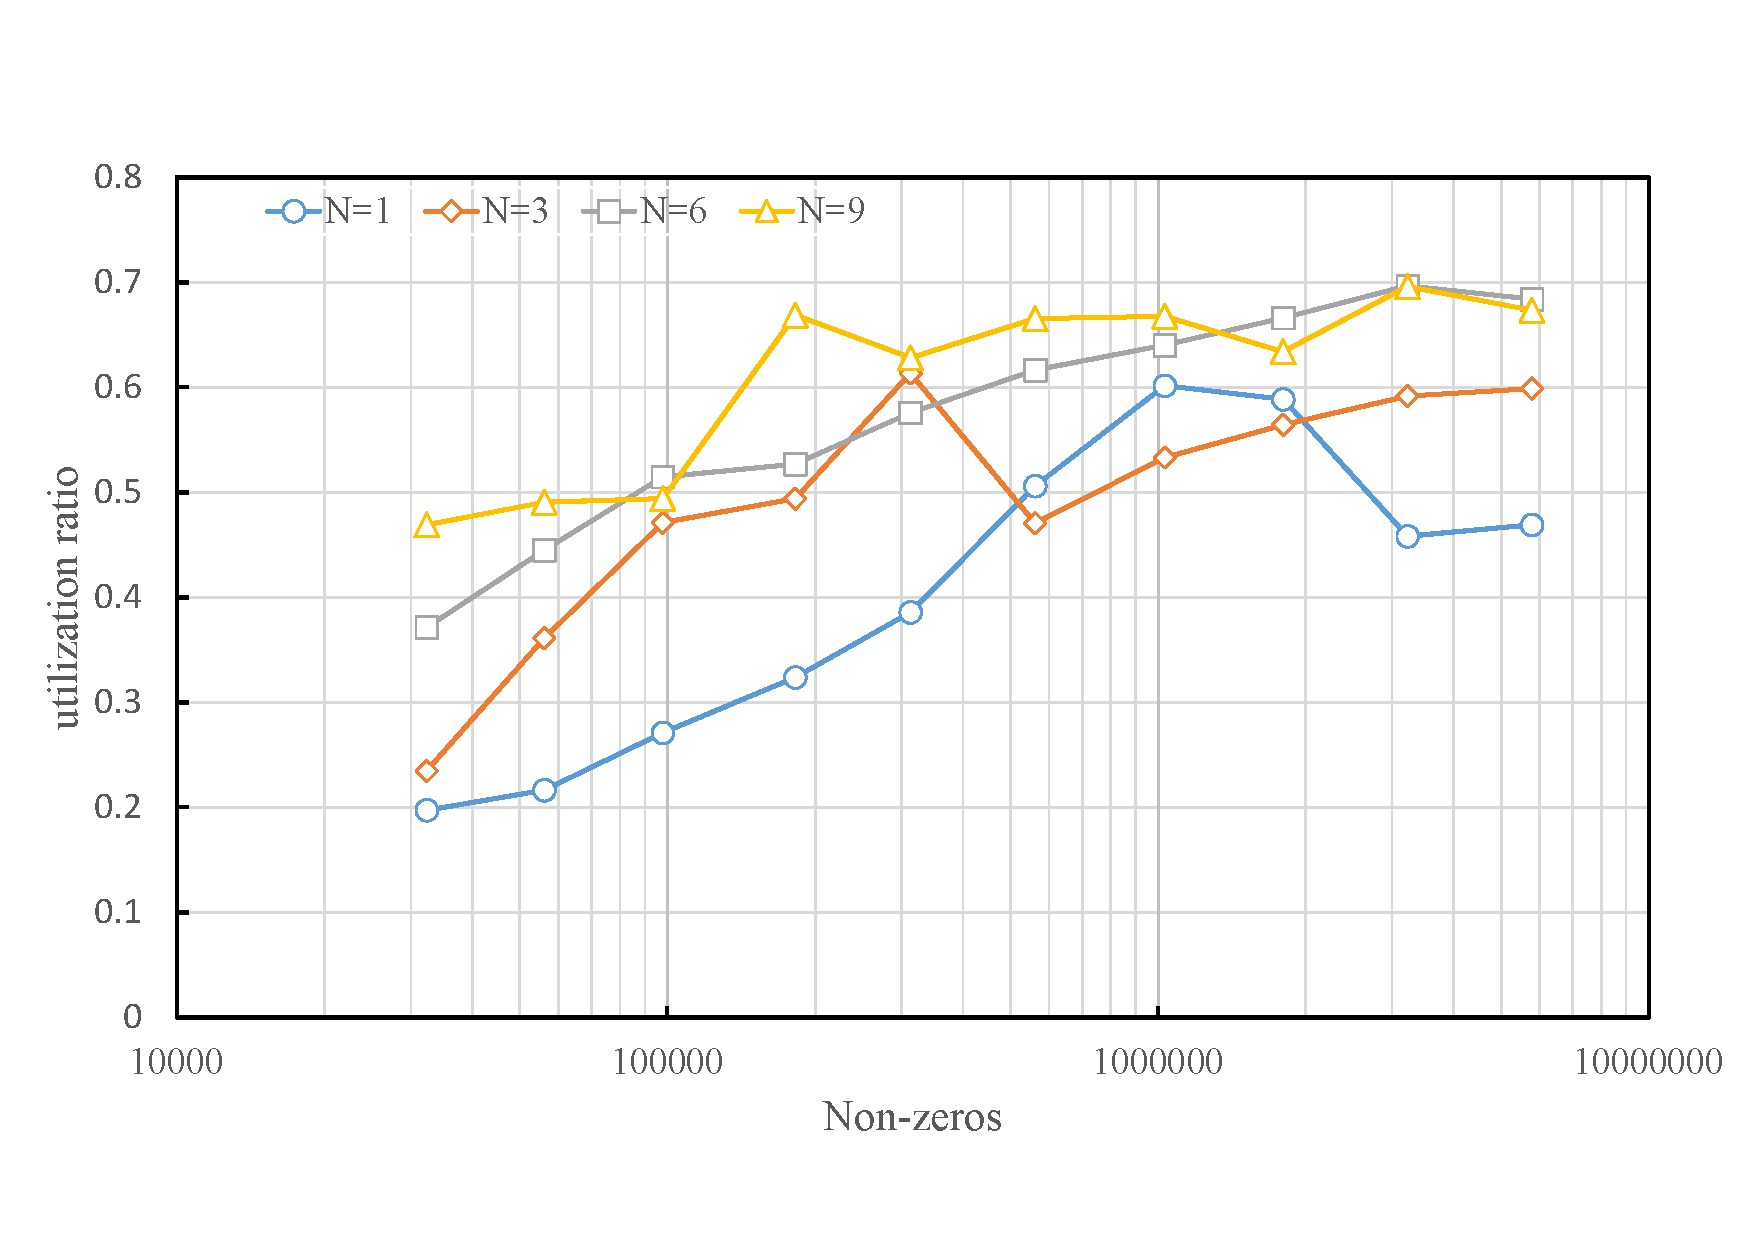
\includegraphics[width=0.45\textwidth]{tau.pdf}}
\caption{The utilization ratio of RSS iterator with COO format.}
\label{tau}
\end{figure}
The data-sets and configuration are identical to the above experiments. It is clear that UNAT can utilize 60\% performance of Sunway processor on average. Considering its universality and compatibility, the performance of UNAT is acceptable and reasonable.

To compare the performance between UNAT API and hand-optimized code, we select a previous research about efficient SpMV on SW26010 processor as a baseline and three sparse matrices from Suit Sparse Matrix Collection. The results are presented in Tab. \ref{comparision}.
% Please add the following required packages to your document preamble:
% \usepackage{multirow}
\begin{table}[]
\centering
\caption{Comparison of UNAT API and hand-optimized code.}
\begin{tabular}{|c|c|c|}
\hline
\multirow{2}{*}{Matrices} & \multicolumn{2}{c|}{GFlops} \\ \cline{2-3} 
                          & UNAT API        & Liu et al.\cite{b8}       \\ \hline
shadow\_water1            & 1.6             & 2.1       \\ \hline
atmosmodd                 & 1.76            & 2.65      \\ \hline
mac\_econ\_fwd500         & 1.82            & 2.72      \\ \hline
\end{tabular}
\label{comparision}
\end{table}
It is clear that UNAT API achieves about 70\% performance compared to the hand-optimized code. Considering the cost resulting from compatibility and generality, the results are quite reasonable.

\section{Conclusion}

In this paper, we present the UNAT abstraction framework for the solution of unstructured grid-based applications. The calculations are separated into three components: connectivity, data-sets and operations. The high-level interfaces are user-friendly and comprehensible.

For Sunway architecture, we design two parallelization strategies in UNAT. In MLB strategy, the unstructured mesh is decomposed into three level: MPI, CG and CPE, corresponding to inter-process, process and thread. For the fine-grained parallel in the CPE level, we collect the discrete data among CPEs and store them continuously in the LDM through RLC. Moreover, we present an "owner-write" model to address the write conflict issue. In RSS strategy, we adopt the accurate data tiling algorithm to enable efficient data caching and design a coloring algorithm to address the race condition problem.

Performance results of two parallelization strategies shows that the speed-up of up to 26$\times$ is reported. We observe that the data layout Struct-of-Arrays (SoA) has better performance than Array-of-Structs (AoS) for these two strategies on Sunway architecture. On the other hand, although we obtain higher speed-ups with the matrix format COO, the benefit is at the cost of redundant computations in some cases. For the convective flux computation of one solver, we obtain the shorter absolute execution time with LDU format. In addition, we propose a method to analyze the utilization ratio of Sunway processor and the results show that UNAT nearly give full play to the performance of Sunway processor with an average utilization ratio of 60\%. The comparison with hand-optimized code indicates that UNAT API achieves reasonable performance with user-friendly API and dozens of code lines.

%% The Appendices part is started with the command \appendix;
%% appendix sections are then done as normal sections
%% \appendix

%% \section{}
%% \label{}

%% For citations use: 
%%       \citet{<label>} ==> Jones et al. [21]
%%       \citep{<label>} ==> [21]
%%

%% If you have bibdatabase file and want bibtex to generate the
%% bibitems, please use
%%
%%  \bibliographystyle{elsarticle-num-names} 
%%  \bibliography{<your bibdatabase>}

%% else use the following coding to input the bibitems directly in the
%% TeX file.
\section{Acknowledgment}

This work was supported by the National Key R\&D Program  of China under Project 2017YFB0203602. The corresponding author is Hu Ren.

\begin{thebibliography}{00}

%% \bibitem[Author(year)]{label}
%% Text of bibliographic item

\bibitem{b1} Diaz, J., Munoz-Caro, C., and Nino, A. (2012). A survey of parallel programming models and tools in the multi and many-core era. IEEE Transactions on parallel and distributed systems, 23(8), 1369-1386.
\bibitem{b2} Mudalige, G. R., Giles, M. B., Reguly, I., Bertolli, C., and Kelly, P. H. J. (2012, May). OP2: An active library framework for solving unstructured mesh-based applications on multi-core and many-core architectures. In 2012 Innovative Parallel Computing (InPar) (pp. 1-12). IEEE.
\bibitem{b3} Mudalige, G. R., Giles, M. B., Thiyagalingam, J., Reguly, I. Z., Bertolli, C., Kelly, P. H., and Trefethen, A. E. (2013). Design and initial performance of a high-level unstructured mesh framework on heterogeneous parallel systems. Parallel Computing, 39(11), 669-692.
\bibitem{b4} Guo, X., Lange, M., Gorman, G., Mitchell, L., and Weiland, M. (2015). Developing a scalable hybrid MPI/OpenMP unstructured finite element model. Computers \& Fluids, 110, 227-234.
\bibitem{b6} Markall, G. R., Slemmer, A., Ham, D. A., Kelly, P. H. J., Cantwell, C. D., and Sherwin, S. J. (2013). Finite element assembly strategies on multi‐core and many‐core architectures. International Journal for Numerical Methods in Fluids, 71(1), 80-97.
\bibitem{b6-6} Gelado, Isaac, and Michael Garland. Throughput-oriented GPU memory allocation. In PPoPP, pp. 27-37. 2019.
\bibitem{b7} Al Farhan, M. A., and Keyes, D. E. (2018). Optimizations of unstructured aerodynamics computations for many-core architectures. IEEE Transactions on Parallel and Distributed Systems, 29(10), 2317-2332.
\bibitem{b8-8} Hadade, I., Wang, F., Carnevale, M., and di Mare, L. (2019). Some useful optimisations for unstructured computational fluid dynamics codes on multicore and manycore architectures. Computer Physics Communications, 235, 305-323.
\bibitem{b9-9} Mudigere, D., Sridharan, S., Deshpande, A., Park, J., Heinecke, A., Smelyanskiy, M., ... and Keyes, D. (2015, May). Exploring shared-memory optimizations for an unstructured mesh CFD application on modern parallel systems. In 2015 IEEE International Parallel and Distributed Processing Symposium (pp. 723-732). IEEE.
\bibitem{b12-12} Miura, N., Koizumi, Y., Take, Y., Matsutani, H., Kuroda, T., Amano, H., ... and Nakamura, H. (2013). A scalable 3D heterogeneous multicore with an inductive ThruChip interface. IEEE Micro, 33(6), 6-15.
\bibitem{b14-14} Economon, T. D., Palacios, F., Alonso, J. J., Bansal, G., Mudigere, D., Deshpande, A., ... and Smelyanskiy, M. (2015). Towards high-performance optimizations of the unstructured open-source SU2 suite. In AIAA Infotech@ Aerospace (p. 1949).
%\bibitem{b15-15} Petit, E., Thébault, L., Möller, N., Dinh, Q., and Jalby, W. (2014, August). Task-based parallelization of unstructured meshes assembly using d\&c strategy. In 2014 IEEE Intl Conf on High Performance Computing and Communications, 2014 IEEE 6th Intl Symp on Cyberspace Safety and Security, 2014 IEEE 11th Intl Conf on Embedded Software and Syst (HPCC, CSS, ICESS) (pp. 874-877). IEEE.
\bibitem{b18-18} Markall, G. R., Slemmer, A., Ham, D. A., Kelly, P. H. J., Cantwell, C. D., and Sherwin, S. J. (2013). Finite element assembly strategies on multi‐core and many‐core architectures. International Journal for Numerical Methods in Fluids, 71(1), 80-97.
\bibitem{b8} Liu, C., Xie, B., Liu, X., Xue, W., Yang, H., and Liu, X. (2018, June). Towards efficient SpMV on sunway manycore architectures. In Proceedings of the 2018 International Conference on Supercomputing (pp. 363-373). ACM.
\bibitem{b21-21} Reguly, I. Z., László, E., Mudalige, G. R., and Giles, M. B. (2016). Vectorizing unstructured mesh computations for many‐core architectures. Concurrency and Computation: Practice and Experience, 28(2), 557-577.
\bibitem{b22-22} Bertolli, C., Betts, A., Kelly, P. H., Mudalige, G. R., and Giles, M. B. (2012, May). Mesh independent loop fusion for unstructured mesh applications. In Proceedings of the 9th conference on Computing Frontiers (pp. 43-52). ACM.
\bibitem{b16} Fang, J., Fu, H., Zhao, W., Chen, B., Zheng, W., and Yang, G. (2017, May). SWDNN: A library for accelerating deep learning applications on sunway taihulight. In 2017 IEEE International Parallel and Distributed Processing Symposium (IPDPS) (pp. 615-624). IEEE.
\bibitem{b9} Davis, T. A., and Hu, Y. (2011). The University of Florida sparse matrix collection. ACM Transactions on Mathematical Software (TOMS), 38(1), 1.
\bibitem{b10} Cook, S. (2012). CUDA programming: a developer's guide to parallel computing with GPUs. Newnes.
\bibitem{b11} Liu, H., Su, X., and Yuan, X. (2018). Accelerating unstructured large eddy simulation solver with GPU. Engineering Computations, 35(5), 2025-2049.
\bibitem{b13} Yuan, X., and Daiguji, H. (2001). A specially combined lower–upper factored implicit scheme for three-dimensional compressible Navier–Stokes equations. Computers and fluids, 30(3), 339-363.
\bibitem{b14} Su, X. (2015). Accurate and robust adaptive mesh refinement for aerodynamic simulation with multi‐block structured curvilinear mesh. International Journal for Numerical Methods in Fluids, 77(12), 747-766.
\bibitem{b15} Roe, P. L. (1981). Approximate Riemann solvers, parameter vectors, and difference schemes. Journal of computational physics, 43(2), 357-372.

\end{thebibliography}
\end{document}

\endinput
%%
%% End of file `elsarticle-template-num-names.tex'.
